%   MSc Business Analytics Dissertation
%   Format based on skeleton template provided as part of module MIS40750
%
%   Title:     Optimising the design of buffer preparation in bioprocessing
%              facilities
%   Author:    Sean Tully
%
%   This file is the top level file for a dissertation.  It contains:
%   - usepackage commands for any packages required
%   - document-wide parameter settings such as textwidth, etc
%   - The text of small items of the frontmatter (title, abstract, etc.) and 
%     backmatter
%
%   Chapter 1: Introduction
%   Chapter 2: Literature Review
%   Chapter 3: Data
%   Chapter 4: Methodology
%   Chapter 5: Results
%   Chapter 6: Discussion
%   Chapter 7: Conclusions
%
%   Change Control:
%   When     Who   Ver  What
%   -------  ----  ---  --------------------------------------------------------
%   01Sep10  SMcG  0.0  Developed MSc Business Analytics Dissertation LaTeX
%                       template
%   06Jun16  ST    0.1  Begun dissertation proper
%

%\documentclass[a4paper,12pt,bibtotoc]{book}
\documentclass[a4paper,12pt,bibtotoc,oneside]{book} %  note no blank pages
\usepackage[utf8]{inputenc}
\usepackage[T1]{fontenc}
\usepackage{makeidx}
\usepackage{amsthm,amsmath,amsfonts,amssymb,latexsym,graphicx,appendix,
subfigure}
\usepackage{algorithm2e}
\usepackage[subfigure]{tocloft} % passing `subfigure' stops clash on compilation
\usepackage{natbib}
\usepackage{lineno}
\usepackage[hyphens]{url}

\usepackage{longtable,tabu}
\usepackage{siunitx}
\sisetup{input-ignore={,},input-decimal-markers={.}}
\usepackage[hidelinks]{hyperref}
\usepackage{doi}
%\usepackage{showframe} % comment this out to remove page layout frames

%   Macros
%   Esp. Theorem styles for amsart/amsbook document classes (currently enabled)
%
%   Sean McGarraghy
%
%   Change Control:
%   Date      Ver  Reason
%   --------  ---  --------------------------------------------------------------
%   12/05/98  0.1  Begun
%

\newcommand*{\Ax}  {Axiom~}
\newcommand*{\Df}  {Definition~}
\newcommand*{\Th}  {Theorem~}
\newcommand*{\Co}  {Corollary~}
\renewcommand*{\Pr}{Proposition~}
\newcommand*{\Lm}  {Lemma~}
\newcommand*{\Rk}  {Remark~}
\newcommand*{\Ex}  {Example~}
\newcommand*{\Exe} {Exercise~}
\newcommand*{\Eq}  {Equation~}
\newcommand*{\dfn} {definition}

\theoremstyle{plain}                 % Default

\newtheorem{thm}{Theorem}[chapter]
\newtheorem{lemma}[thm]{Lemma}
\newtheorem{lem}[thm]{Lemma}
\newtheorem{propn}[thm]{Proposition}
\newtheorem{pr}[thm]{Proposition}
\newtheorem{prp}[thm]{Propn.}
\newtheorem{cor}[thm]{Corollary}
\newtheorem{fact}[thm]{Fact}
\newtheorem{conj}[thm]{Conjecture}
\newtheorem{claim}{Claim}[]

\theoremstyle{definition}

\newtheorem{dm}{}  % Dummy theorem name for numbering only, ind. of section
\newtheorem{dmy}[thm]{}  % Dummy theorem name for numbering only
\newtheorem{defn}[thm]{Definition}
\newtheorem{ex}[thm]{Example}
\newtheorem{exe}[thm]{Exercise}

\theoremstyle{remark}

\newtheorem{rmk}[thm]{Remark}
\newtheorem{notn}[thm]{Notation}
\newtheorem{note}[thm]{Note}
\newtheorem{cmt}[thm]{Comment}
\newtheorem{case}[thm]{Case}
\newtheorem{intr1}[thm]{Introduction}
\newtheorem{intro}[thm]{Introduction}

\newenvironment{pf}{\vspace{-4pt}\noindent\begin{proof}}{\end{proof}\vspace{2pt}
}




%   General LaTeX Declarations (try -adobe-courier-medium-r-normal--18-180-75-75-m-110-iso8859-2)
%
%   Sean McGarraghy
%
%   Change Control:
%   Date      Ver  Reason
%   --------  ---  --------------------------------------------------------------
%   12/02/98  0.1  Begun
%

% Where to hyphenate words LaTeX doesn't know

\hyphenation{neigh-bour-hood neigh-bour-hoods}
\hyphenation{Bel-field}

% Short commands for italic, bold etc fonts

\newcommand*{\tr}[1]{\textrm{#1}}
\newcommand*{\ti}[1]{\textit{#1}}
\newcommand*{\tb}[1]{\textbf{#1}}
\newcommand*{\ts}[1]{\textsl{#1}}
\newcommand*{\tc}[1]{\textsc{#1}}
\newcommand*{\mr}[1]{\mathrm{#1}}
\newcommand*{\mb}[1]{\mathbf{#1}}
\newcommand*{\tth}[1]{{\slshape #1}}
\newcommand*{\df}[1]{\textbf{#1}}      % put the thing being defined in bold

\newcommand*{\bs}{$\backslash$}
\newcommand*{\ol}[1]{\overline{#1}}
\newcommand*{\cnj}[1]{\overline{#1}}
\newcommand*{\nth}[1]{\ensuremath{{#1}^{\textrm{th}}}}% superscripted `th' for counting
\newcommand*{\nst}[1]{\ensuremath{{#1}^{\textrm{st}}}}% superscripted `st' for counting
\newcommand*{\nnd}[1]{\ensuremath{{#1}^{\textrm{nd}}}}% superscripted `nd' for counting
\newcommand*{\nrd}[1]{\ensuremath{{#1}^{\textrm{rd}}}}% superscripted `rd' for counting

% commonly occurring text in Maths documents

\newcommand*{\eg}  {e.\,g.~}
\newcommand*{\ie}  {i.\,e.~}
\newcommand*{\ff}  {\textrm{if and only if }}
\newcommand*{\A}   {\textrm{ for all }}
\newcommand*{\all} {\textrm{ for all }}
\renewcommand*{\AA}{\ensuremath{\forall~}}
\newcommand*{\E}   {\textrm{ there exists }}
\newcommand*{\EE}  {\ensuremath{\exists~}}
\newcommand*{\st}  {\textrm{ such that }}
\newcommand*{\sta} {\textrm{ such that, for all }}
\newcommand*{\tfae}{the following are equivalent}
\newcommand*{\Tfae}{The following are equivalent}
\newcommand*{\wrt} {with respect to }
\newcommand*{\wolog}{without loss of generality}
\newcommand*{\Wolog}{Without loss of generality}
\newcommand*{\ftsoc}{for the sake of contradiction}
\newcommand*{\resp}{respectively}
\newcommand*{\RHS} {right hand side}
\newcommand*{\LHS} {left hand side}
\newcommand*{\Pf}  {\noindent\tb{Proof: }}            % for backwards compatibility only
\newcommand*{\eop} {~~\vrule height 5 pt width 5 pt depth 0 pt\relax}
\newcommand*{\QED} {\mbox{}\hspace{\fill}\eop}

\newcommand*{\fn}  {function}
\newcommand*{\vsp} {vector space}

\newcommand*{\ind} {independent}
\newcommand*{\dep} {dependent}
\newcommand*{\lcmb}{linear combination}
\newcommand*{\lind}{linearly independent}
\newcommand*{\ldep}{linearly dependent}
\newcommand*{\di}  {dimension}
\newcommand*{\fd}  {finite-dimension}
\newcommand*{\cp}  {characteristic polynomial}
\newcommand*{\de}  {determinant}
\newcommand*{\evl} {eigenvalue}
\newcommand*{\evc} {eigenvector}
\newcommand*{\sle} {system of linear equations}
\newcommand*{\ERO} {elementary row operation}
\newcommand*{\ECO} {elementary column operation}
\newcommand*{\repn}{representation}

\newcommand*{\UCD} {University College Dublin} 

\newcommand*{\itema}[1][a]{\item[(\emph{#1})]} 
\newcommand*{\ita}[1][a]{(\emph{#1})} 

% Math Roman abbreviations e.g. Gal(), Aut() etc.

\newcommand*{\len}{\ensuremath{\operatorname{length}}}% 
\newcommand*{\rank}{\ensuremath{\operatorname{rank}}} % RANK of matrix/linear map
\newcommand*{\nll}{\ensuremath{\operatorname{nullity}}} % NULLity of linear map
\newcommand*{\diag}{\ensuremath{\operatorname{diag}}} % DIAGonal matrix
\newcommand*{\cond}{\ensuremath{\operatorname{cond}}} % CONDition number
\newcommand*{\sign}{\ensuremath{\operatorname{sign}}} % SIGNature
\newcommand*{\sgn} {\ensuremath{\operatorname{sgn}}}  % SiGN of permutation
\newcommand*{\imp}{\ensuremath{\mathbin\Rightarrow}}  % IMPlies sign
\renewcommand*{\Im}{\ensuremath{\operatorname{Im}}}   % IMage (of a map)
\newcommand*{\zv} {\ensuremath{\mathbf{0}}}           % Zero vector
\newcommand*{\zs}[1]{\ensuremath{{#1}^{-1}(0)}}       % Zero Set of function #1
\renewcommand*{\i}[1]{\ensuremath{{#1}^{-1}}}         % Inverse of geezer #1

% spacing/heading commands

\newcommand*{\cpb}{\vspace{\fill}\pagebreak}          % Clean PageBreak inside paragraph
\newcommand*{\cb}{\hspace*{\fill}\\*[\medskipamount]} % Clean Break inside paragraph
\newcommand*{\cbb}{\hspace*{\fill}\\[\medskipamount]} % Clean Break, may have page Break
\newcommand*{\cbs}{\hspace*{\fill}\\*[\smallskipamount]} % Small Clean Creak inside paragraph
\newcommand*{\cbbs}{\hspace*{\fill}\\[\smallskipamount]} % Small Clean Creak, may have page break
\newcommand*{\cbl}{\hspace*{\fill}\\*}                % No gap Clean Break inside paragraph
\newcommand*{\cbbl}{\hspace*{\fill}\\}                % No gap Clean Break, may have page break

\newcommand*{\qt}[1]{\ensuremath{\quad\text{#1}\quad}}
\newcommand*{\qqt}[1]{\ensuremath{\qquad\text{#1}\qquad}}

\newcommand*{\subhead}[1]{  
            \begin{center}
            \tb{#1}
            \end{center}\\*}


% Various inclusion, ideal, equivalence, mapping symbols

%\newcommand*{\squig}{\sim\!\sim\!\rightarrow}  % old definition
\newcommand*{\eqv} {\ensuremath{\mathbin\Leftrightarrow}}  % EQuiValence sign
\newcommand*{\app} {\ensuremath{\rightarrow}}          % APProaches/tends to (limit)
\newcommand*{\map} {\ensuremath{\longrightarrow}}      % set MAPs to (long arrow)
\newcommand*{\tmap}[1]{\ensuremath{
                      \stackrel{\ssk{#1}}{\map} }}    % scriptsize #1 atop ---> arrow
\newcommand*{\mpt}{\ensuremath{\longmapsto}}          % element maps to (long arrow with bar)
\newcommand*{\tmpt}[1]{\ensuremath{
                               \stackrel{#1}{\mpt}}}  % scriptsize #1 atop |--> arrow
\newcommand*{\cng}{\ensuremath{\equiv}}               % CoNGruent to 
\newcommand*{\rel}{\ensuremath{\sim}}                 % single tilde RELation sign
\newcommand*{\nul}{\ensuremath{\emptyset}}            % NULl set 
\newcommand*{\su} {\ensuremath{\subset}}              % SUbset of
\newcommand*{\se} {\ensuremath{\subseteq}}            % Subset of/Equal to
\newcommand*{\sne}{\ensuremath{\subsetneqq}}          % Subset of but Not Equal to
\newcommand*{\sm} {\ensuremath{\smallsetminus}}       % set difference (Set Minus)
\newcommand*{\la} {\ensuremath{\langle}}              % Left Angle bracket
\newcommand*{\ra} {\ensuremath{\rangle}}              % Right Angle bracket
\newcommand*{\du} {\ensuremath{\dot{\cup}}}           % Disjoint Union (dot over cup sign)
\newcommand*{\rt}{\right}
\newcommand*{\lt}{\left}
\newcommand*{\oo}{\ensuremath{\infty}}                % oo = infinity
\newcommand*{\fp}[3]{\ensuremath{{#1}:{#2}\map{#3}}}  % Function/maP f:A--->B
\newcommand*{\ma}[3]{\ensuremath{{#1}:\R^{#2}\map\R^{#3}}} % MAp f:R^n--->R^m
\newcommand*{\lma}[4][]{linear map{#1} \ma{#2}{#3}{#4}} % linear map(s) f:R^n--->R^m
\newcommand*{\cpd}[1][A]{\ensuremath{\det({#1}-\l I)}} % char poly eg det(A-lI)

% Logic and proof
\newcommand*{\LT} {\texttt{T}}
\newcommand*{\LF} {\texttt{F}}
\newcommand*{\NOT}{\mathop\mathrm{not}}
\newcommand*{\AND}{\mathbin\mathrm{and}}
\newcommand*{\OR} {\mathbin\mathrm{or}}

% Binomial coefficient
\newcommand*{\bin}[2]{\ensuremath{\binom{#1}{#2}}}

% Binomial coefficient (textstyle i.e. Small font)
\newcommand*{\sbin}[2]{\ensuremath{\tbinom{#1}{#2}}}

% Binomial coefficient (displaystyle i.e. Big font)
\newcommand*{\bbin}[2]{\ensuremath{\dbinom{#1}{#2}}}

% derivatives
\newcommand*{\dd}[1]{\ensuremath{\displaystyle{\frac{d}{d{#1}}}}}

\newcommand*{\polyn}[3][n]{\ensuremath{{#3}_0+{#3}_1{#2}+\cdots+{#3}_{#1}{#2}^{#1}}}

% MATRICES

% two commonly used building blocks for matrices

% identity matrix
\newcommand*{\idmat}{\ensuremath{ 
1      & 0      & \cdots & 0       \\
0      & 1      & \cdots & 0       \\
\vdots & \vdots & \ddots & \vdots  \\
0      & 0      & \cdots & 1          } }

% matrix consisting of zeros
\newcommand*{\zeromat}{\ensuremath{ 
0      & 0      & \cdots & 0       \\
\vdots & \vdots & \ddots & \vdots  \\
0      & 0      & \cdots & 0          } }

% matrix consisting of asterisks
\newcommand*{\astmat}{\ensuremath{ 
*      & *      & \cdots & *       \\
\vdots & \vdots & \ddots & \vdots  \\
*      & *      & \cdots & *          } }

% Greek letters - abbreviations

\renewcommand*{\a}{\ensuremath{\alpha}}
\renewcommand*{\b}{\ensuremath{\beta}}
\newcommand*{\g}{\ensuremath{\gamma}}
\renewcommand*{\d}{\ensuremath{\delta}}
\newcommand*{\e}{\ensuremath{\varepsilon}}
\newcommand*{\z}{\ensuremath{\zeta}}
\newcommand*{\h}{\ensuremath{\eta}}
\renewcommand*{\th}{\ensuremath{\vartheta}}
%\newcommand*{\io}{\ensuremath{\iota}}
\renewcommand*{\k}{\ensuremath{\kappa}}
\renewcommand*{\l}{\ensuremath{\lambda}}
\newcommand*{\m}{\ensuremath{\mu}}
\newcommand*{\n}{\ensuremath{\nu}}
\renewcommand*{\r}{\ensuremath{\rho}}
\newcommand*{\s}{\ensuremath{\sigma}}
\renewcommand*{\t}{\ensuremath{\tau}}
\renewcommand*{\u}{\ensuremath{\upsilon}}
\newcommand*{\f}{\ensuremath{\varphi}}
\renewcommand*{\c}{\ensuremath{\chi}}
\newcommand*{\x}{\ensuremath{\xi}}
\newcommand*{\p}{\ensuremath{\psi}}
\renewcommand*{\o}{\ensuremath{\omega}}

\newcommand*{\G}{\ensuremath{\Gamma}}
\newcommand*{\D}{\ensuremath{\Delta}}
\newcommand*{\T}{\ensuremath{\Vartheta}}
\renewcommand*{\L}{\ensuremath{\Lambda}}
\renewcommand*{\L}{\ensuremath{{\textstyle{\bigwedge}}}}
%\newcommand*{\Si}{\ensuremath{\Sigma}}
\newcommand*{\U}{\ensuremath{\Upsilon}}
\newcommand*{\F}{\ensuremath{\Phi}}
\renewcommand*{\P}{\ensuremath{\Psi}}
\renewcommand*{\O}{\ensuremath{\Omega}}


% Math mode blackboard and calligraphic (script) letters

\newcommand*{\N}{\ensuremath{\mathbb{N}}}
\newcommand*{\Z}{\ensuremath{\mathbb{Z}}}
\newcommand*{\Q}{\ensuremath{\mathbb{Q}}}
\newcommand*{\R}{\ensuremath{\mathbb{R}}}
\newcommand*{\C}{\ensuremath{\mathbb{C}}}
\renewcommand*{\H}{\ensuremath{\mathbb{H}}}
\newcommand*{\FF}{\ensuremath{\mathbb{F}}}

\newcommand*{\sA}{\ensuremath{\mathcal{A}}}
\newcommand*{\sB}{\ensuremath{\mathcal{B}}}
\newcommand*{\sC}{\ensuremath{\mathcal{C}}}
\newcommand*{\sD}{\ensuremath{\mathcal{D}}}
\newcommand*{\sE}{\ensuremath{\mathcal{E}}}
\newcommand*{\sF}{\ensuremath{\mathcal{F}}}
\newcommand*{\sG}{\ensuremath{\mathcal{G}}}
\newcommand*{\sH}{\ensuremath{\mathcal{H}}}
\newcommand*{\sI}{\ensuremath{\mathcal{I}}}
\newcommand*{\sJ}{\ensuremath{\mathcal{J}}}
\newcommand*{\sK}{\ensuremath{\mathcal{K}}}
\newcommand*{\sL}{\ensuremath{\mathcal{L}}}
\newcommand*{\sM}{\ensuremath{\mathcal{M}}}
\newcommand*{\sN}{\ensuremath{\mathcal{N}}}
\newcommand*{\sO}{\ensuremath{\mathcal{O}}}
\newcommand*{\sP}{\ensuremath{\mathcal{P}}}
\newcommand*{\sQ}{\ensuremath{\mathcal{Q}}}
\newcommand*{\sR}{\ensuremath{\mathcal{R}}}
\newcommand*{\sS}{\ensuremath{\mathcal{S}}}
\newcommand*{\sT}{\ensuremath{\mathcal{T}}}
\newcommand*{\sU}{\ensuremath{\mathcal{U}}}
\newcommand*{\sV}{\ensuremath{\mathcal{V}}}
\newcommand*{\sW}{\ensuremath{\mathcal{W}}}
\newcommand*{\sX}{\ensuremath{\mathcal{X}}}
\newcommand*{\sY}{\ensuremath{\mathcal{Y}}}
\newcommand*{\sZ}{\ensuremath{\mathcal{Z}}}


\linespread{1.25}         % spacing between lines
\parindent0pt             % no paragraph indentation
\parskip\smallskipamount  % small space between paragraphs

%\setlength{ \topmargin      }{  -1cm }
%\setlength{ \textheight     }{  24cm }
\setlength{ \textwidth      }{  14cm }
\setlength{ \oddsidemargin  }{ 1.0cm }
%\setlength{ \oddsidemargin  }{ 1.5cm }
\setlength{ \evensidemargin }{ 1.0cm }

\numberwithin{equation}{section}
\numberwithin{figure}{chapter}

\pagestyle{plain} % just puts a page number at the bottom of each page

\makeindex % generates the index entries (unsorted: need to run makeindex from
%            the command line to sort them)

\includeonly{
  preface,
  ch1,
  ch2,
  ch3,
  ch4,
  ch5,
  ch6,
  ch7,
  appendix1, 
  appendix2, 
  glossary,
  notation
}

\begin{document}

\frontmatter 

\title
{Optimising the design of buffer preparation in bioprocessing facilities}

\author{Sean Tully, M.A. (\emph{Cantab.}), M.Eng.}

\maketitle

{\normalsize 
\vfill
\begin{center} 
\textup{A dissertation submitted to University College Dublin in part
fulfilment of the requirements of the degree of M.Sc. in Business Analytics}
\end{center}
\vfill
\begin{center} 
Michael Smurfit Graduate School of Business,
\end{center}
\begin{center} 
University College Dublin
\end{center}
\vfill
\begin{center} 
\textit{August, 2017}
\end{center}
\vfill
\begin{center} 
\textup{Supervisor: Prof. M. O'Neill}
\end{center}
\vfill
\begin{center} 
\textup{Head of School: Professor Ciar\'an \'O h\'Ogartaigh}
\end{center}
\vfill
}

\thispagestyle{empty}

\clearpage

%% Dedication
\chapter*{Dedication} 
To \ldots


%% Table of Contents
\cleardoublepage
\tableofcontents
\clearpage

%% List of Figures (Illustrations)
\listoffigures\addcontentsline{toc}{chapter}{List of figures}
\clearpage

%% List of Tables
\listoftables\addcontentsline{toc}{chapter}{List of tables}

%% List of Algorithms (if any): need to \usepackage{algorithm2e} for nice 
%  algorithm layout and this command
%\listofalgorithms\addcontentsline{toc}{chapter}{List of algorithms}


%% Preface
%   MSc Business Analytics Dissertation
%   Format based on skeleton template provided as part of module MIS40750
%
%   Title:     Optimising the design of buffer preparation in bioprocessing
%              facilities
%   Author:    Sean Tully
%
%   Preface
%
%   Change Control:
%   When     Who   Ver  What
%   -------  ----  ---  --------------------------------------------------------
%   06Jun16  ST    0.1  Begun 
%

\chapter*{Preface}

\begin{quote}
The cold smell of potato mould, the squelch and slap

Of soggy peat, the curt cuts of an edge

Through living roots awaken in my head.

But I've no spade to follow men like them.

Between my finger and my thumb

The squat pen rests.

I'll dig with it.

\hspace{2cm}--- Seamus Heaney, \emph{Digging}
\end{quote}

This thesis was motivated by \ldots

% Introduction?
We begin in Chapter 1 with a short overview of \ldots 

% Business Background?
In Chapter 2 we \ldots 

% Literature Review?
Chapter 3 introduces \ldots 

% Methodology?
In Chapter 4, the \ldots 

% Results --- experimental, survey, etc
We explore in Chapter 5 \ldots 

% Discussion?
Chapter 6 examines \ldots 

% Conclusions and future work?
Finally, in Chapter 7, we \ldots{} 
and indicate some possible avenues for further research following on from the
ideas introduced in this thesis.

\vspace{2em}

University College Dublin \hfill Sean Tully \\
\today 



%% Acknowledgements (including permissions and other credits).
\chapter*{Acknowledgements}

I would like to thank my supervisor, Prof. Michael O'Neill.

I would also like to thank David Lynch for the helpful feedback on the write-up
and Dr. Paula Carroll for her advice on linear programming.

%% Abstract
%%\begin{abstract}
\chapter*{Abstract} 
This dissertation seeks to define the problem of buffer vessel selection in
bioprocessing facility design.
It succeeded in modelling the problem mathematically, as a series of linear
constraints on binary and real variables.
The problem was then implemented such that it can be solved using one of a
range of mixed-integer linear programming packages.
Equipment time utilisation plots were designed to visualise the results.
The models were trialled on both random and real-world data and found to be
robust.
The complexity of the models and time taken for solution were investigated.
Scope for further work was outlined in terms of some additional features or
constraints that could be added to the model.
%%\end{abstract}

%%   List of important abbreviations (including special fonts, e.g.,
%    \ {\tt fixed width} for program code)
 
% Bulk of thesis. line numbers in arabic numerals, 1, 2, 3, ...
\mainmatter 

\linespread{1.3} % adjust line spacing (if desired)

%   MSc Business Analytics Dissertation
%   Format based on skeleton template provided as part of module MIS40750
%
%   Title:     Optimising the design of buffer preparation in bioprocessing
%              facilities
%   Author:    Sean Tully
%
%   Chapter 1: Introduction
%
%   Change Control:
%   When     Who   Ver  What
%   -------  ----  ---  --------------------------------------------------------
%   06Jun16  ST    0.1  Begun 
%

\chapter{Introduction}\label{C.intro}

\begin{quote}
Well I don't think we're \emph{for} anything. We're just products of evolution.
You can say, `Gee, your life must be pretty bleak if you don't think there's a
purpose.' But I'm anticipating having a good lunch.

\hspace{2cm}--- James Watson, \emph{in conversation with Richard Dawkins}
\end{quote}

\section{Bioprocessing}\label{SS.bioproc}

Before the advent of biotechnology, most therapeutics (medicines) were what are
now termed \emph{small molecule} drugs. The pharmaceutical industry was
concerned with the synthesis of these products via predominantly chemical
processes, such as reaction, distillation and  crystallisation.  Small molecule
drugs typically consist of tens or hundreds of atoms, such as paracetamol, which
has a molar mass of approximately 151 g/mol, or aspirin (acetylsalicylic acid),
which has a molar mass of approximately 180 g/mol.

With the advent of recombinant D.N.A technology, biochemists gained
the ability to re-program the D.N.A. of simple biological microorganisms such as
\textit{Escherichia coli} and, eventually, mammalian cells, such as those of the
Chinese Hamster (\textit{Cricetulus griseus}).  The genetic structure of these
cells could be modified to produce complex molecules, which had previously
proved difficult or impossible to synthesise by any other means.  The
biopharmaceutical industry is concerned with the synthesis of therapeutics via
such biological pathways.  These products are known by various names, such as
\emph{biopharmaceuticals}, \emph{protein therapeutics} or, colloquially, as
\emph{biotech drugs}.

The first protein therapeutic to be synthesised on a large scale using 
biological pathways was insulin, which is a hormone used to regulate metabolism
and is administered to individuals suffering from diabetes.  Human insulin has a
molar mass of approximately 5808 g/mol.  It was not possible to commercially
synthesise insulin chemically and it was initially produced by extracting the
hormone from the pancreases of mammals such as cows or pigs.  In 1978, 
scientists working at  the American company Genentech (now a subsidiary of the
Swiss pharmaceutical company F. Hoffmann-La Roche AG) successfully modified 
cells of \textit{E. coli} to produce insulin and this synthetic insulin was
first brought to market in 1982.

The industry that has grown up around the production of biopharmaceuticals is 
known as the \emph{biopharmaceutical industry}, or, colloquially, as the
\emph{biotech} or \emph{biopharma} industry.  A report by strategy consultants
McKinsey \& Company \citep{Otto:2014} estimates that the biopharmaceutical 
market had global revenues of \$163 billion per annum and was worth 20\% of the
overall pharmaceutical market.  \citet{Otto:2014} also note that large-scale
biopharmaceutical manufacturing facilities typically cost in the region of
``\$200 million to \$500 million or more'' to build.

\section{Bioprocess Engineering}\label{SS.bioproceng}

\citet{Schaschke:2014} defines bioprocess engineering as ``A specialist branch
of (chemical) engineering that involves the design and operation of processes
used for the production of biological products such as foods, pharmaceuticals,
and biopolymers.''  The design of a large-scale biopharmaceutical facility
typically takes about two years and requires a multidisciplinary team of
engineers and scientists.

\section{Upstream and Downstream}\label{SS.updown}

A complete facility typically starts with frozen vials of cells (the 
\emph{working cell bank}) and finishes with the final formulated product in
either bulk form or filled into its final packaging \textit{e.g.} syringes.
Facilities are nominally divided into \emph{upstream} and \emph{downstream} 
sections.
The upstream section is predominantly concerned with the expansion of cells
from a small vial into progressively larger tanks of \emph{media}.  
The final stage of this growth occurs in the \emph{production bioreactor}, 
wherein the conditions can be altered to encourage the cells to produce the 
target protein.

At the interface between upstream and downstream lies the \emph{harvest}
section. In the harvest section, some initial separation is performed to begin
to isolate the target protein from the contents of the batch (which at this
point include cells, cell waste, growth media, antibiotics and myriad other
contaminants).  At the end of the harvest section, all traces of the host cells
should be removed and the batch is said to be \emph{cell-free}.  Different
interpretations exist in the industry as to where the upstream-downstream split
occurs, but it usually is defined as being at some point in the harvest section.

Downstream processing is concerned with taking the cell-free but otherwise 
contaminated batch and purifying it through a series of orthogonal processes.
Such processes can include filtration, ultrafiltration/diafiltration 
(\emph{UF/DF}), chromatography, reaction, virus inactivation and formulation.
At the end of downstream processing, a batch should consist of formulated bulk
product, ready to be filled into its final packaging for delivery. The final 
fill/finish steps often occur in a separate, sterile facility.

\section{Buffers and Media}\label{SS.buffmed}

Both upstream and downstream sections require large volumes of aqueous solutions
to be prepared and stored.  Solutions used upstream are typically referred to as
\emph{media} and those used downstream are typically referred to as
\emph{buffers}.  Strictly speaking, media refers to the solutions of nutrients
into which cells are expanded, but the term is usually used to encompass all
other upstream solutions, such as acids and bases anti-foam used in the
bioreactors.  Strictly speaking, a chemist would define a buffer as a solution
which maintains its pH over a wide range of concentrations.  Most solutions used
downstream do indeed meet this criteria, but the term \emph{buffers} is
generally used as a catch-all for all solutions used in the downstream section.
A typical process to produce a \emph{monoclonal antibody} (a common family of 
protein therapeutics) can use tens or hundreds of litres of buffers and media 
per litre volume in the production bioreactor.  Typical large-scale production
bioreactor volumes for such processes are in the range 10,000--30,000 litres.
Each batch may use in the region of 20--40 different buffers and media.

\section{Buffers and Media Preparation}\label{SS.buffmedprep}

One of the reasons for the catch-all definitions of \emph{buffers} and
\emph{media} in the section above is to do with segregation.
The upstream and downstream sections of the plant are segregated to prevent
cross-contamination.
As a result, there are typically two main areas where solutions are prepared.
Buffers are prepared in an area called \emph{buffer preparation}, for use
downstream and media are prepared in an area called \emph{media preparation},
for use upstream.
There may also be a separate area for preparing sterile buffers for the final
formulation, again to reduce the possibility of contamination and ensure
sterility is maintained.
In both media and buffer preparation, one vessel is used to prepare the solution
and then it is typically sterile filtered into either a hold vessel or the
destination vessel.

\section{Design of Buffer Preparation Areas}\label{SS.buffprepdes}

For a given product, a production process is defined at laboratory scale.  The
definition of key parameters at laboratory scale can allow process engineers to
generate a production-scale mass balance.  This mass balance provides, amongst
other things, lists of all buffers and media required to make a batch.  Two
complex optimisation problems now emerge; how do we design the buffer and media
preparation areas?  For media, the problem is relatively easy to solve with some
trial and error, since there are typically only about 10 media used per batch
and they often differ vastly in scale; the initial bioreactor may be 20 litres
in volume and the production bioreactor may be 20,000 litres in volume.  Because
of this, the sizing of preparation vessels usually proceeds by picking a vessel
capable of preparing the largest medium, defining a minimum fill volume and
seeing what else can be prepared in it, then defining another vessel, and so on
until sufficient vessels are defined.  Media hold vessels, if required, may be 
similarly defined.  The design of media preparation is usually relatively
insensitive to schedule.

The problem of designing a buffer preparation area is more difficult to solve.
There may be 20 or more different buffer compositions.  Often each buffer is
used multiple times in the same operation or multiple times across multiple
operations.  In operations such as chromatography, somewhere in the region of
5--10 buffers may be needed in rapid succession.  They tend to be of similar 
volumes, so an efficient solution will look to maximise the number of buffers
prepared in a given preparation vessel.  Since they may be needed in rapid
succession, this then involves a requirement for multiple hold vessels so
some buffers can be made ahead of time.  Where buffers are required for multiple
steps in an operation or across multiple operations, is it best to perform
many preparations, or few?  Additionally, is it best to hold the buffer
in many separate hold vessels, allowing them to be individually freed up more
quickly, or is it better to consolidate and minimised the number of vessels?
Defining success in the design of buffer preparation is also difficult.
There exist trade-offs between efficiency and flexibility, capital and 
operating costs, and many other factors such as installed area, installed 
volume, operability, layout/adjacency, pipework complexity and cleanability.

Due to the high salt concentrations in some buffers, they can prove corrosive
to the commonly used grades of stainless steel, such as 316L.  Such buffers
may have to be prepared or held in vessels made from expensive alloys such as
AL-6XN\textsuperscript{\textregistered}, which is about 3.5 times more
expensive than 316L, or a steel from the
Hastelloy\textsuperscript{\textregistered} family, which can be eight or more
times more expensive than 316L.
Ideally, the use of these alloys should be minimised.

Another factor is the use of disposable technology.  Buffer preparation, at
scales of up to 3,000 litres, can be carried out in disposable sterile bags,
rather than vessels.  These have a higher consumable cost but are faster to turn
around between preparations and reduce the utilisation of cleaning equipment.
Similarly, buffers can be held in disposable bags at volumes of up to 5,000
litre.  Development of disposables technology is currently rapid and the
available sizes and product ranges are increasing each year, so much so that 
the state of the art has often moved on between the finish of the detailed
design of a facility and the start of the first saleable production batch.

\section{Problem Definition}\label{SS.probdef}
\begin{figure}
    \centering
    \includegraphics[angle=0,scale=1]{./figures/buffer_pfd.pdf}
    \caption{Buffer preparation schematic}
    \label{fig.pfd}
\end{figure}


%TODO
\textbf{TODO: Rewrite this section}

The task of designing a buffer preparation area is complex.
Current workflows are largely based on trial-and-error methods using process
engineering scheduling software.  
Typically, a conservatively large array of vessels is chosen and the schedule
is run.  
If there is an individual vessel for each task, the schedule will resolve
easily, but the capital and space requirements will be onerous.
Via trial-and-error, individual vessels may be removed or resized and
the schedule re-run to see if it can be resolved.  
After some iteration, it becomes difficult or impossible to remove or reduce
the vessels any further and resolve the schedule.
At this point, iteration stops.
% TODO: Pseudocode for this methodology 
In the early feasibility or concept stages of a project, this process is
cumbersome, the end points are poorly defined and any development of the
underlying process which varies the volumes required may necessitate starting
the optimisation again from scratch.
An additional factor is that a working solution may exist for a given
configuration, but the scheduling software is unable to resolve the problem,
giving a false negative. 
The scheduling tools used for the process tend to be deterministic, rather than
stochastic (although some sensitivity analysis is usually built in as an 
add-on); this makes it difficult to have confidence that a working schedule can
handle the real-world batch-to-batch variability inherent in a process that has
living cells at its heart.S

A more streamlined methodology for solving this optimisation problem is
required and this dissertation is concerned with developing such a methodology
and a software tool to implement it.
The aim is to start with a reduced or basic case, including a number of
simplifying assumptions, and develop a working tool to schedule the operations
in buffer preparation and to vary the size and number of vessels and the 
preparation strategy to optimise the process with respect to some metric.
One a working framework has been developed, additional constraints can be added
and simplifications can be removed to provide a better approximation of 
real-world conditions.

Success will be defined both in terms of the ability for the software tool to
provide an optimum solution and the speed at which it can be implemented
relative to other methods or benchmarks.

The business imperatives are twofold.
For an engineering consultancy, the ability to rapidly, accurately and
repeatably solve such problems gives a competitive edge, which can be used to
win more business and to deliver designs more cheaply.  For a biopharmaceutical
client, optimising this problem results in cost savings and having a well
defined methodology for doing so gives confidence that an in-progress design is
indeed optimal and robust.


%   MSc Business Analytics Dissertation
%   Format based on skeleton template provided as part of module MIS40750
%
%   Title:     Optimising the design of buffer preparation in bioprocessing
%              facilities
%   Author:    Sean Tully
%
%   Chapter 2: Literature Review
%
%   Change Control:
%   When     Who   Ver  What
%   -------  ----  ---  --------------------------------------------------------
%   06Jun16  ST    0.1  Begun 
%

\chapter{Literature Review}\label{C.litreview}

\begin{quote}
It was long before I got at the maxim, that in reading an old mathematician you
will not read his riddle unless you plough with his heifer; you must see with
his light, if you want to know how much he saw.

\hspace{2cm}--- Augustus de Morgan, \emph{letter to W. R. Hamilton}
\end{quote}

\section{Introduction}\label{S.intro2}

In this chapter, recent papers related to the design of bioprocess facilities
are reviewed.  This is followed by the review of papers related to solving
similar problems in related industries.  Finally, papers relating to more
general methodologies for solving scheduling and optimisation problems are
reviewed.

\subsection{Bioprocess Facility Design}\label{SS.bioprocdes}

Current bioprocess facility design leverages software packages for creating mass
balances and for schedule simulation.  The mass balance tool
\emph{SuperPro Designer\textsuperscript{\textregistered}} 
and the scheduling tool \emph{SchedulePro\textsuperscript{\textregistered}}
from Intelligen, Inc. (\emph{Scotch Plains, New Jersey, U.S.A.}) are examples of
software packages that are widely used, particularly by American firms.
The \emph{INOSIM} family of software from INOSIM Software GmbH
\emph{Dortmund, Germany} is used particularly by German and Swiss firms.

\citet{Petrides:2014} outline a workflow for 
the design of a ``typical'' monoclonal antibody facility using 
\emph{SuperPro Designer\textsuperscript{\textregistered}} and
\emph{SchedulePro\textsuperscript{\textregistered}} and compares the use of
these packages with other methodologies.
While this paper does touch on buffer preparation,
it does not elaborate on a strategy for optimising the area, stating:
\begin{quote}In most real processes, buffer scheduling is considerably more
complex and challenging because of the larger number of buffers required for a
typical process (more than twenty), the shared use of pipe segments and transfer
panels, as well as constraints imposed by the limited availability of labor.
\end{quote}
\citet{Petrides:2014} cite an earlier paper by \citet{Toumi:2010} which also
looks at design of a facility for monoclonal antibody production.
\citet{Toumi:2010} also mention the difficulty of optimising the sizing and 
selection of buffer equipment, but do not outline a methodology for doing so.

\citet{Dietz:2008} outlines a genetic algorithm approach to optimising the 
design of protein production facilities, which is capable of dealing with
imprecise demands.  It is primarily looking at the specification of the main
process equipment and mass balance and it does not touch on buffer preparation.

No mentions could be found of methodologies for optimising buffer preparation in
bioprocess facility design.

\subsection{Facility Design Optimisation in the Process Industry}
\label{SS.fdopi}
Casting the net wider to the pharmaceutical, chemical and other process
industries yields several articles that deal with similar families of problems.

Of particular relevance to buffer preparation are efforts to simulate tank farm
design \citep{Al-Otaibi:2004, Stewart:2005, Sharda:2009, Terrazas-Moreno:2012}.
Tank farms commonly exist in large pharmaceutical, chemical and oil \&
gas facilities and consist of arrays of tens of tanks that are usually dedicated
to particular chemicals or products, but may me multi-use.  These tanks are used
to support the main process being carried out in the facility, similar to the
role of buffer hold vessels.  There are a great deal of papers that deal with
optimising throughput or productivity of existing tank farms or existing batch
processes, but very little articles relating to the optimisation of the design
of such processes.

\citet{Al-Otaibi:2004} describes efforts to optimise the design of a tank farm
for the oil \& gas industry using both linear programming and Monte Carlo
simulation methods.  Their brief magazine article does not provide any detail on
how the simulations were carried out.

\citet{Stewart:2005} cite the work of \citet{Al-Otaibi:2004} and outline a
method for optimising tank farm design using Monte Carlo simulation.  They
mention the use of a software tool called \emph{GRTMPS} from 
\emph{Haverley Systems, Inc., Houston, Texas, U.S.A}, supported by \emph{Excel}
spreadsheet software and \emph{Access} database software
(\emph{Microsoft Inc, Redmond, Washington, U.S.A}).
Again, this is a short magazine article.  It indicates that the scheduling 
produced useful results but does not give any technical detail as to how the
simulation was carried out.

\citet{Sharda:2009} outline the use of the discrete-event simulation tool
\emph{Arena\textsuperscript{\textregistered}} from
\emph{Rockwell Automation, Inc., Milwaukee, Wisconsin, U.S.A.} to optimise the 
utilisation of existing tank farm facilities and cite the work of
\citet{Sharda:2009}

\citet{Terrazas-Moreno:2012}, citing \citet{Stewart:2005} and 
\citet{Sharda:2009} provide a far more detailed description of efforts to
optimise tank farm operations using mixed integer linear programming 
\emph{MILP}.  Their work looks at optimising both schedule and tank selection, 
but is not strictly designed with the design of the facility itself, but rather
the optimal operation of a designed facility.

The work of \citet{Terrazas-Moreno:2012} provides some useful information on
techniques that could be applied to solve the problem of buffer preparation
area design, namely MILP and process scheduling.  Branching out further into
these fields yields more relevant literature.

\citet{Dedieu:2003} suggests a hybrid apprach using genetic
algorithms and discrete-event simulation to address the problem of 
multiobjective batch plant design.

In \citet{Cavin:2004, Cavin:2005}, tabu search is discussed as a methodology to
optimise the design of multi-purpose batch plants.

\subsection{Simulation and Optimisation}\label{SS.simopt}

Casting the net wider still to look at techniques for solving generalised
scheduling and optimisation problems yields far more material, but further 
research is required to decide which techniques, if any, are relevant to the 
problem at hand.

There are two aspects to optimising the design.  The first aspect is scheduling,
as the ability to make a tank do more than one task will depend on the times
at which the tasks must (or may) occur.  The second aspect is selecting the
optimal sizes and numbers of vessels, which can be seen as a combinatorial
optimisation problem.

In his seminal 1957 paper, George Dantzig \nocite{Dantzig:1957} outlines several
types of combinatorial optimisation problems, one of which is the
\emph{knapsack problem}.  This problem relates to finding the most valuable
selection of objects that can be carried in a knapsack, subject to a total
weight limit, given a selection of candidate items, each having a weight and a 
value.
A whole range of knapsack-type problems have been researched in the intervening
period.  Detailed descriptions of the most common problems and the research 
carried out over the half century following Dantzig's paper are given by 
\citet{Korte:2012} and \citet{Martello:1990}.

One knapsack-type problem that may be of particular relevance is the bin-packing
problem.  \citet{Martello:1990} describes the bin packing problem as one in
which there are a number of items with associated weights and a number of bins
with associated capacities.  The aim is to each item to a bin so that the weight
capacity of the bin is not exceeded and the number of bins is minimised.
A number of algorithms for both exact and approximate solutions of the
bin-pakcing problem have been developed. \citet{Korte:2012} state that the
bin-packing problem is strongly $\mathcal{NP}$-hard, indicating that efforts
should be taken to minimise the sample space when dealing with optimising vessel
selection.

\citet{Bettinelli:2010} investigates a particular variant of the bin packing
problem where there is a minimum filling constraint.  This is an important
consideration in vessel selection, usually some minimum fill level,
\textit{e.g.} 20--30\% is defined so that the impeller in the vessel remains
sumbmerged during the mixing process and to reduce the volume of cleaning
solutions or water required to clean the vessel as a fraction of the volume of 
buffer produced.

In terms of process scheduling methodologies, a number of papers exist in the 
field of chemical engineering \citep{Ahmed:2000},

\citet{Ahmed:2000} states that the general process planning problem is also
$\mathcal{NP}$-hard.

A detailed synopsis of scheduling methodologies applicable to the chemical 
and process industries is given by \citet{Harjunkoski:2014}.

\subsection{Literature review summary}\label{litsum}
It can be seen that the area of design of buffer preparation facilities in the
sphere of bioprocessing is not a current area of research and directly relevant
papers are not readily avialable. This body of research aims to formulate a 
framework for such design by draw on more generalised methodologies for solving
scheduling and optimisation problems, for which more detailed research exists.
Examples of such methodologies are given above, particularly in the works by
\citep{Harjunkoski:2014} and \citet{Korte:2012}

%   MSc Business Analytics Dissertation
%   Format based on skeleton template provided as part of module MIS40750
%
%   Title:     Optimising the design of buffer preparation in bioprocessing
%              facilities
%   Author:    Sean Tully
%
%   Chapter 3: Data
%
%   Change Control:
%   When     Who   Ver  What
%   -------  ----  ---  --------------------------------------------------------
%   06Jun16  ST    0.1  Begun
%

\chapter{Data}\label{C.data}

\begin{quote}
We have some freedom in setting up our personal standards of beauty, but it is
especially nice when the things we regard as beautiful are also regarded by
other people as useful.

\hspace{2cm}--- Donald Knuth, \emph{Computer Programming as an Art}
\end{quote}

\section{Introduction}\label{S.intro3}
This chapter will outline the requirements for input data.

For modelling a single process, a typical data-set consists of three distinct
files.
The first file is a table of data relating to the available selection of
vessels.
The second file is a table of data relating to parameters specific
to each buffer.
The third file comprises a collection of global parameters
that apply to all vessels and/or buffers.

One particular example, based on some randomly generated data, is used
throughout this chapter to illustrate the relevant data formats.

\section{Vessel Data}\label{S.vesseldata}

\begin{table}[h!]
    \centering
    \caption{Vessel data for random example}
    \label{tbl.vessel}
    \begin{tabular}{l | r | r}
        names & volumes & costs\\
        & $V_{m}$ (l) & $c_{m}$ (--)\\\hline
        \SI{1000}{\litre} & \SI{1000.0}{} & \SI{63.10}{}\\
        \SI{2000}{\litre} & \SI{2000.0}{} & \SI{95.64}{}\\
        \SI{3000}{\litre} & \SI{3000.0}{} & \SI{121.98}{}\\
        \SI{4000}{\litre} & \SI{4000.0}{} & \SI{144.96}{}\\
        \SI{5000}{\litre} & \SI{5000.0}{} & \SI{165.72}{}\\
        \SI{6000}{\litre} & \SI{6000.0}{} & \SI{184.88}{}\\
        \SI{8000}{\litre} & \SI{8000.0}{} & \SI{219.71}{}\\
        \SI{10000}{\litre} & \SI{10000.0}{} & \SI{251.19}{}\\
        \SI{12000}{\litre} & \SI{12000.0}{} & \SI{280.83}{}\\
        \SI{16000}{\litre} & \SI{16000.0}{} & \SI{333.02}{}\\
        \SI{18000}{\litre} & \SI{18000.0}{} & \SI{357.41}{}\\
        \SI{20000}{\litre} & \SI{20000.0}{} & \SI{380.73}{}\\
        \SI{22000}{\litre} & \SI{22000.0}{} & \SI{403.14}{}\\
        \SI{25000}{\litre} & \SI{25000.0}{} & \SI{435.28}{}\\
        \SI{30000}{\litre} & \SI{30000.0}{} & \SI{485.59}{}\\
    \end{tabular}
\end{table}

The vessel data will contain several parameters for each available vessel size,
$m \in M$.
A vessel data-set will contain entries for $\mathcal{M}$ vessel sizes:
\begin{equation}
    m \in M; \quad M = \left\{ 0, 1, 2, \ldots, m, \ldots, \left(
    \mathcal{M} - 1 \right) \right\}
\end{equation}
\begin{equation}
    \mathcal{M} = |M|
\end{equation}

Typically, when designing a large-scale production facility, buffer preparation
vessel volumes range from \SI{1000}{\litre} to \SI{30000}{\litre}.

When ordering such a vessel, the stated size of the vessel is usually a nominal
volume, which will differ from the liquid fill volume and may also differ from
the maximum working volume.
It is usual to round the stated or nominal volume to the nearest thousand
litres.

For the purposes of this study, it is assumed that, for each vessel $m \in M$,
the specified vessel volume, $V_{m}$ is the maximum working volume (in litres)
of the vessel, which is taken to be the maximum volume of buffer which can be
prepared in that vessel.

Vessels will also have a minimum working volume.
It is usual to assume a minimum fill ratio of about 30\% of the vessel volume.
This limitation arises due to the minimum agitation volume of the impeller in
the vessel.
For the purposes of this simulation, the minimum fill ratio is a global
parameter.
It may be possible to specify a value of minimum fill ratio for every vessel
size, but this level of detail is typically neither required nor available.

For each vessel, $m \in M$, a (relative) cost, $c_{m}$, must also be defined.
Note that absolute costs are not required to find the vessel selection that
minimises costs.
Vessel costs tend not to scale linearly with volume.

Sample vessel data are given in \hyperref[tbl.vessel]{Table \ref*{tbl.vessel}}.
In this table, the cost value for each vessel size has been estimated by
raising the vessel volume (in litres) to a power of 0.6 and rounding to two
decimal places.
Note that the vessel volumes, $V_{m}$, are equal to the nominal volumes
indicated in the `names' column.  The contents of the `names' column are
treated as identifiers and are not used in any calculation.
It is not uncommmon to have values of $V_{m}$ slightly larger than their
respective named (nominal) volumes; a vessel with a nominal volume of e.g.\
\SI{1000}{\litre} will be capable of holding at least \SI{1000}{\litre}, with
the precise maximum working volume being a function of the vessel geometry.

\section{Buffer Data}\label{S.bufferdata}

\begin{table}[h!]
    \centering
    \caption{Buffer data for random example}
    \label{tbl.buffer}
    \begin{tabular}{l | c | c | c}
        names & required volumes & use start times & use durations\\
        & $U_{n}$ (l) & $t_{\mathit{USE},n}^{*}$ (h) 
        & $\Delta t_{\mathit{USE},n}$
        (h)\\ \hline
        \text{Buffer \#1} & \SI{24427.13}{} & \SI{76.23}{} & \SI{20.56}{}\\
        \text{Buffer \#2} & \SI{5487.29}{} & \SI{0.21}{} & \SI{49.77}{}\\
        \text{Buffer \#3} & \SI{2588.36}{} & \SI{25.78}{} & \SI{24.56}{}\\
        \text{Buffer \#4} & \SI{7102.05}{} & \SI{46.79}{} & \SI{27.77}{}\\
        \text{Buffer \#5} & \SI{1020.87}{} & \SI{87.7}{} & \SI{36.58}{}\\
        \text{Buffer \#6} & \SI{19508.79}{} & \SI{35.52}{} & \SI{58.53}{}\\
        \text{Buffer \#7} & \SI{23073.55}{} & \SI{42.26}{} & \SI{39.71}{}\\
        \text{Buffer \#8} & \SI{25454.10}{} & \SI{48.38}{} & \SI{43.47}{}\\
        \text{Buffer \#9} & \SI{24088.67}{} & \SI{4.18}{} & \SI{55.41}{}\\
        \text{Buffer \#10} & \SI{3172.46}{} & \SI{48.31}{} & \SI{23.27}{}\\
        \text{Buffer \#11} & \SI{24752.71}{} & \SI{76.38}{} & \SI{45.80}{}\\
        \text{Buffer \#12} & \SI{13445.31}{} & \SI{73.93}{} & \SI{34.25}{}\\
    \end{tabular}
\end{table}

The buffer data will contain several parameters for each buffer to be prepared,
$n \in N$.
A buffer data-set will contain entries for $\mathcal{N}$ buffers:
\begin{equation}
    n \in N; \quad N = \left\{ 0, 1, 2, \ldots, n, \ldots, \left(
    \mathcal{N} - 1 \right) \right\}
\end{equation}
\begin{equation}
    \mathcal{N} = |N|
\end{equation}
For each buffer, $n \in N$, the data-set will contain, at a minimum, its
required preparation volume (in litres), $U_{n}$.

If nothing was known about the scheduling of the production process, a simple
simulation could be carried out without scheduling.
Such a simulation would assume a fixed duration for all operations in the
preparation procedure and would require knowledge of the cycle time and an
additional parameter representing the maximum utilisation ratio of the
preparation vessels (see \hyperref[S.parameters]{Section \ref*{S.parameters}}).

For a complete model, with scheduling, we also need to know when each buffer
is first required by the process, and the duration for which it is required.

Sample buffer data are given in \hyperref[tbl.buffer]{Table \ref*{tbl.buffer}}.
\hyperref[fig.explanatory]{Figure \ref*{fig.explanatory}} gives an overview of
data and parameters related to scheduling, which are detailed in the reaminder
of this section and in \hyperref[S.parameters]{Section \ref*{S.parameters}}.
The plot in \hyperref[fig.explanatory]{Figure \ref*{fig.explanatory}} is
termed an \emph{equipment time utilisation} plot; in this instance it just
shows the preparation and hold procedures for a single buffer.
This style of plot is covered in more detail in
\hyperref[C.results]{Chapter \ref*{C.results}}, where similar plots can be used
to visually display a working steady-state schedule for a feasible solution.

\begin{figure}
    \centering
    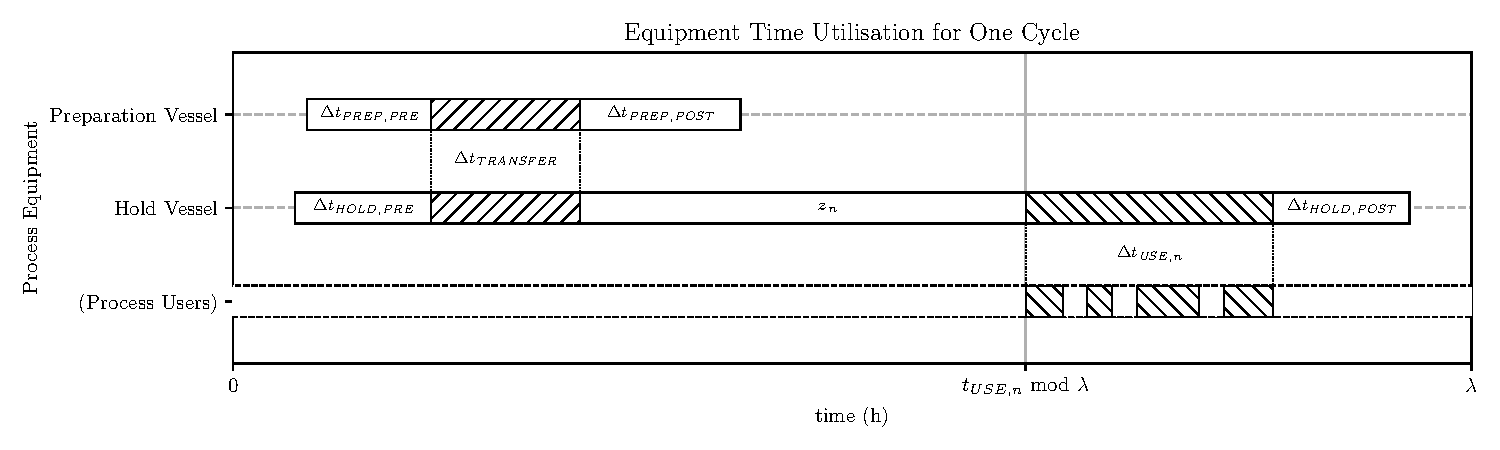
\includegraphics[angle=0,scale=0.55]{./figures/explanatory.pdf}
    \caption{Equipment time utilisation for a single buffer}
    \label{fig.explanatory}
\end{figure}

For each buffer, $n \in N$, its (unnormalised) time of first use,
$t_{\mathit{USE},n}^{*}$, is the time when the process draws the first drop of
buffer from its hold vessel.
This time is relative to some batch datum, e.g.\ the start of the batch or the
start of downstream processing.
The choice of datum is unimportant once it is consistently used. 
The model deals with steady-state processing, so we are interested in a 
single-cycle window.
As a result, we want to normalise $t_{\mathit{USE},n}^{*}$ with respect to the
cycle time, $T$.
Accordingly, we define:
\begin{equation}
    t_{\mathit{USE},n} = t_{\mathit{USE},n}^{*} \enspace \text{mod} \enspace 
    T \quad \forall n \in N
\end{equation}
Note that the random data generator used to produce the data in 
\hyperref[tbl.buffer]{Table \ref*{tbl.buffer}} produces values for 
$t_{\mathit{USE},n}^{*}$ that are already normalised, but for the real-world
examples discussed in \hyperref[C.results]{Chapter \ref*{C.results}}, 
$t_{\mathit{USE},n}^{*}$ may be unnormalised.

For each buffer, $n \in N$, its duration of first use,
$\Delta t_{\mathit{USE},n}$, is the duration from when the process draws the
first drop of buffer from its hold vessel to when it finishes drawing the last
drop of buffer from the same vessel.
Note that a process may draw buffer discontinuously from a hold vessel, e.g.\ a
cleaning buffer may be drawn from its hold vessel for a few minutes at the end
of a chromatography procedure and may not be required again until near the end
of another chromatography procedure a day or two later, but may not be required
at all in the intervening period.
Note the use of the general convention that \emph{durations} are denoted by
$\Delta t$, whereas \emph{times} (relative to some datum) are denoted by $t$.
It is assumed that all times and durations are in hours.

For each buffer, $n$, $\Delta t_{\mathit{USE},n}$ must be sufficiently less
than the cycle time so that there is opportunity to \emph{turn around} its hold
vessel (i.e.\ sufficient time must exist after use of the buffer to clean and
sterilise the vessel, receive the subsequent batch of buffer and hold for a
sufficient duration before use of that buffer is required by the subsequent
batch).

\section{Parameters}\label{S.parameters}

In addition to the buffer-specific and vessel-specific data detailed above,
some global parameters are required to specify the problem.
For the random example, these parameters are tabulated in
\hyperref[tbl.parameters]{Table \ref*{tbl.parameters}} and are described in
more detail hereafter.

\begin{table}[h!]
    \centering
    \caption{Global parameters for random example}
    \label{tbl.parameters}
    \begin{tabular}{l | l | r | c}
        symbol & short description & value & unit\\ \hline
        $T$ & process cycle time & 96.0 & h\\
        $\Delta t_{\mathit{PREP,PRE}}$ & prep pre duration & 12.0 & h\\
        $\Delta t_{\mathit{PREP,POST}}$ & prep post duration & 1.5 & h\\
        $\Delta t_{\mathit{TRANSFER}}$ & transfer duration & 2.0 & h\\
        $\Delta t_{\mathit{HOLD,PRE}}$ & hold pre duration & 8.0 & h\\
        $\Delta t_{\mathit{HOLD,POST}}$ & hold post duration & 1.5 & h\\
        $\Delta t_{\mathit{HOLD,MIN}}$ & minimum hold duration & 12.0 & h\\
        $\Delta t_{\mathit{HOLD,MAX}}$ & maximum hold duration & 60.0 & h\\
        $f_{\mathit{MINFILL}}$ & minimum fill ratio & 0.3 & --\\
        $f_{\mathit{UTIL}}$ & maximum utilisation ratio & 0.8 & --\\
    \end{tabular}
\end{table}

The first parameter sepcified is the cycle time, $T$.  We are concerned
with the steady-state operation of the process, so the cycle time can be
thought of as the duration from some fixed point in one batch to the same
fixed point in the subsequent batch.
The cycle time is typically some multiple of 24 hours.
This is for reasons of operability; it is easier for staff if a given task
occurs at the same time of the day for each batch.
Note that it is not our objective to seek to minimise the cycle time.
A well-designed facility should be bottlenecked at the production bioreactor,
so the cycle time is a function of the production process and not the buffer
preparation area.

In the model, the preparation and hold procedures are both broken into a number
of operations.
The durations of most of these operations are specified as global parameters.
It is unlikely that detailed timings will be available at the early stages of
design, so specifying some conservative global parameters provides a model that
is easy to comprehend and validate.
In reality, operations such as filling a vessel with water will scale with
buffer bolume and operations such as cooldown of a vessel after steaming will
scale with vessel volume.
This degree of granularity could be added as a future model enhancement.

The following durations are specified as global parameters:

The parameter $\Delta t_{\mathit{PREP,PRE}}$ is the duration of all operations
in the preparation procedure prior to the transfer of buffer to the buffer hold
vessel.  
This may include pressure testing, steam-in-place (SIP) and cooldown, although
these tasks are not always carried out on preparation vessels.
The period will include the charging of WFI, the charging of other liquids
and/or solids, and time for mixing the buffer.
It may also include some time for sampling or testing and adjustment of the
buffer.

The parameter $\Delta t_{\mathit{PREP,POST}}$ is the duration of all operations
in the preparation procedure that take place after the transfer of the buffer
to the buffer hold vessel is complete.
This is typically just comprised of the clean-in-place (CIP) of the vessel.
CIP involves a separate piece of equipment, the CIP skid, which circulates
cleaning fluids (detergents and/or acids, bases) through the vessel and some of
its attached pipework.

The parameter $\Delta t_{\mathit{PREP,POST}}$ is the duration of the transfer
of buffer from the preparation vessel to the hold vessel, via a sterile filter.
Although this varies with the buffer volume, the relationship is not that
straightforward.
As buffer and vessel volumes increase, a change in pipe diameter or pump size
may be appropriate, giving large step changes to the transfer duration.
Accordingly, a conservative global parameter for transfer duration is
appropriate for early-stage design.

The parameter $\Delta t_{\mathit{HOLD,PRE}}$ is the duration of all operations
in the hold procedure prior to the commencement of receipt of buffer from the
preparation vessel.
This typically includes pressure testing, SIP and cooldown.

The parameter $\Delta t_{\mathit{HOLD,POST}}$ is the duration of all operations
in the hold procedure that take place after the last use of buffer by the
process is complete.
Like $\Delta t_{\mathit{PREP,POST}}$, this is primarily comprised of a CIP of
the respective vessel.

Looking at \hyperref[fig.explanatory]{Figure \ref*{fig.explanatory}}, the one
symbol not yet mentioned is the buffer hold duration, $\boldsymbol{z}_{n}$.
Note that this is a decision variable, and not a parameter; it is discussed in
more detail in \hyperref[C.methodology]{Chapter \ref*{C.methodology}}.
The buffer hold duration is the duration that spans from the end of the
transfer into the buffer hold vessel until the start of the first use of the
buffer by the process.
As will be described in 
\hyperref[C.methodology]{Chapter \ref*{C.methodology}},
we place some bounds on this duration and express these bounds as a pair of
global parameters.
The parameter $\Delta t_{\mathit{HOLD,MIN}}$ defines the minimum allowabe
duration of the buffer hold operation.
In practice, the operators of a plant do not want to schedule buffer
preparations so that the transfer is complete moments before the buffer is
required by the process, as any delays at this stage could imapct production.
A value, typically in the range of several hours to one day, can be specified
to ensure that buffers are prepared with some flexibility to handle delays.
At the other end of the scale, buffers may expire and the global variable 
$\Delta t_{\mathit{HOLD,MIN}}$ is defined to set a maximum allowable hold
duration.

When selecting a vessel, a minimum fill ratio, $f_{\mathit{MINFILL}}$ is
defined to ensure that a vessel isn't selected that is far too big for the
buffer being prepared. The rationale for this was mentioned in
\hyperref[S.vesseldata]{Section \ref*{S.vesseldata}}.

Finally, the utilisation ratio, $f_{\mathit{UTIL}}$, places an upper limit on
how busy a preparation vessel is allowed to be.
In the absence of detailed buffer scheduling information, this may represent an
`engineering factor' to account for unforseeable scheduling clashes.
If detailed scheduling information is available, the ratio can be set to unity
to effectively remove its influence as a constraint, or the ratio could be
maintained at some value less than one to allow for some overhead in the
design.

\section{Data Sources}\label{S.sources}

\subsection{Random Data}\label{SS.randomdata}
The buffer data in \hyperref[tbl.buffer]{Table \ref*{tbl.buffer}} were randomly
generated.  
The parameters in \hyperref[tbl.parameters]{Table \ref*{tbl.parameters}} and
the vessel data in \hyperref[tbl.vessel]{Table \ref*{tbl.vessel}} are typical
figures based on the author's experience of designing and optimising
bioprocessing facilities.

A function was developed to generate random buffer data.
The function requires four inputs; the number of buffers required,
$\mathcal{N}$, the minimum duration ratio, $f_{\mathit{MINUSE}}$, the maximum
duration ratio, $f_{\mathit{MAXUSE}}$, and a `parameters' dataset.
The function generates the required number of buffers, each with
$t_{\mathit{USE},n}^{*}$ uniformly distributed in the range
$0 < t_{\mathit{USE},n}^{*} < T$. Note that, for the random data, this means
that $t_{\mathit{USE},n}^{*} = t_{\mathit{USE},n}$, i.e.\ the random use
times are already normalised.
The use durations, $\Delta t_{\mathit{USE},n}$ are uniformly distributed and
depend on several parameters so that the model is feasible.  The feasible range
may be further scaled back using $f_{\mathit{MINUSE}}$ and
$f_{\mathit{MAXUSE}}$ to ensure values are credible, i.e.
$f_{\mathit{MINUSE}} \times T < \Delta t_{\mathit{USE},n} < f_{\mathit{MAXUSE}}
 \times \Delta t_{\mathit{FEAS}}$
where
\begin{equation}
    \Delta t_{\mathit{FEAS}} = T - \left( 
    \Delta t_{\mathit{HOLD,PRE}}
    + \Delta t_{\mathit{TRANSFER}}
    + \Delta t_{\mathit{HOLD,MIN}}
    + \Delta t_{\mathit{HOLD,POST}} \right)
\end{equation}

These values are bound below by the minimum duration ratio times the cycle time

\subsection{Real-World Data}\label{SS.realdata}
Real-world data sets are based on mass balances and scheduling simulations
performed by the author for biopharmaceutical clients.
Since these processes are highly confidential, the data has been obfuscated in
several ways.
Firstly, the buffers are all given terse names, such as `Buffer \#1', and are
in no particular order.
Secondly, the buffer volumes may be scaled but only to a degree that does not
affect vessel selection.
Thirdly, the (normalised) duration parameters may all be scaled by a common
factor.
These changes serve to make the data unrecognisable but do not affect vessel
selection or scheduling (save for scaling the time axis).





%   MSc Business Analytics Dissertation
%   Format based on skeleton template provided as part of module MIS40750
%
%   Title:     Optimising the design of buffer preparation in bioprocessing
%              facilities
%   Author:    Sean Tully
%
%   Chapter 4: Methodology
%
%   Change Control:
%   When     Who   Ver  What
%   -------  ----  ---  --------------------------------------------------------
%   06Jun16  ST    0.1  Begun
%

\chapter{Methodology}\label{C.methodology}

\begin{quote}
Just as the largest library, badly arranged, is not so useful as a very
moderate one that is well arranged, so the greatest amount of knowledge, if not
elaborated by our own thoughts, is worth much less than a far smaller volume
that has been abundantly and repeatedly though over.  For only by universally
combining what we know, by comparing every truth with every other, do we fully
assimilate our own knowledge and get it into our power.

\hspace{2cm}--- Arthur Schopenhauer, \emph{On Thinking for Oneself}
\end{quote}

\section{Introduction}\label{S.intro4}
At first glance, the pathway to solving the vessel selection problem was
unclear.
There are two aspects to the problem; scheduling and selection.

For the scheduling aspect of the problem, initial concepts involved finding an
API to one of the commercial scheduling packages.
One initial concept included developing an algorithm or heuristic to
intelligently guess at possible vessel selections, and pass these into a
scheduling model which could be repeatedly be solved using a commercial
scheduling package to find an optimum selection.
It became evident that this concept would be cumbersome and computationally
difficult.

The vessel selection problem appears to be a close relative of a number of
classic \textbf{NP}-hard problems in the `bin-packing' genre so another
concept was to look at how such problems were solved and see if any
methodologies could be adapted to suit the problem at hand.
It was noted that bin-packing problems, as well as some scheduling problems,
such as job-shop scheduling, were solved using mixed-integer linear
programming (MILP) -- see, e.g.\ \citet{Martello:1990}, \citet{Taha:2017}.

The focus thus centred on formulating the problem as a MILP problem.
Firstly, the problem was described mathematically.
Next, attention was focused on the method of solution.

\section{Slots}\label{S.slots}

To model the problem as an MILP problem, we must introduce the concept of
\emph{slots}.
Noting that there is a buffer hold vessel for each buffer, it is evident that
a feasible but inefficient solution could involve installing a dedicated,
suitably sized, preparation vessel for each hold vessel.
Any solution involving more than this number of preparation vessels cannot
be optimal.
As a result, we have an upper limit of $N$ on the number of required
preparation vessels.
The model is thus constructed with $P$ \emph{slots}, where
\begin{equation}
    P = N.
\end{equation}
A slot, $p \in \mathcal{P}$, is a notional space which may be occupied by a
vessel, or may be empty;
\begin{equation}
    p \in \mathcal{P}; \quad \mathcal{P} = \left\{ 0, 1, 2, \ldots, p, \ldots,
    \left( P - 1 \right) \right\}
\end{equation}
and
\begin{equation}
    P = |\mathcal{P}|.
\end{equation}
Note that slots do not have any physical significance, i.e.\ in a real-world
facility, floor space is assigned to physical vessels, rather than notional
slots.

\section{Objective Function}\label{S.objfn}

The vessel selection problem may be described as a series of linear
constraints.
These constraints are applied to find the optimum value of an objective
function, which we seek to minimise.
The primary objective function is the total cost of vessels.
We find this by summing the vessel costs for all vessels present in slots.
Recall that the vessel data set contains entries for $\mathcal{M}$ vessel
sizes, each of which has an associated cost, $c_{m}$.

We now introduce the first decision variable, $\boldsymbol{y}_{mp}$.
This a binary decision variable with dimensions $M \times P$.
Note that binary decision variables may only take the values 0 and 1, i.e.
\begin{equation}
    \boldsymbol{y}_{mp} \in \left\{ 0, 1 \right\} \quad \forall m \in
    \mathcal{M} \quad \forall p \in \mathcal{P}.
    \label{eq.y}
\end{equation}
The possible states of $\boldsymbol{y}_{mp}$ may be described thus:
\begin{equation}
    \boldsymbol{y}_{mp} =
    \begin{cases}
        1 \implies \text{instance of vessel $m$ in slot $p$}\\
        0 \implies \text{otherwise.}
    \end{cases}
\end{equation}
We can now describe the objective function, which gives an expression for the
objective function \emph{value}, $\boldsymbol{Z}$.
The primary objective is to minimise $\boldsymbol{Z}$.
\begin{equation}
    \boldsymbol{Z} = \sum_{m \in \mathcal{M}} \sum_{p \in \mathcal{P}} 
    c_m \boldsymbol{y}_{mp}, \quad \boldsymbol{Z} \in \mathbb{R}; \;
    \boldsymbol{Z} \ge 0.
    \label{eq.objfn}
\end{equation}

\section{Basic Model}\label{S.basicprob}

A small number of constraints need to be applied to arrive at the simplest
variant of the problem.
Additional constraints may then be added to make the model more detailed or
realistic.
The basic model requires no information on when each buffer is required by the
process and only provides a rough estimation of vessel requirements as a
result.
The complete model, detailed in
\hyperref[S.completemodel]{Section \ref*{S.completemodel}}, exists as an
extension of the basic model.

\subsection{Buffers Dedicated to Slots}\label{SS.constr1}

The first constraint to be added is the limitation that a buffer must be
prepared in exactly one slot.
This constraint means that we must prepare each buffer once per cycle
and also that the buffer is always prepared in the same slot, i.e.\ slot
selection is identical for every cycle.

We introduce a new binary decision variable, $\boldsymbol{x}_{np}$, which takes
a value of 1 if buffer $n$ is prepared in slot $p$, and takes a value of 0
otherwise, i.e.
\begin{equation}
    \boldsymbol{x}_{np} \in \left\{ 0, 1 \right\} \quad \forall n \in 
    \mathcal{N} \quad \forall p \in \mathcal{P}.
    \label{eq.x}
\end{equation}
Note that $\boldsymbol{x}_{np}$ has dimensions of $N \times P$.
The possible states of $\boldsymbol{x}_{np}$ may be described thus:
\begin{equation}
    \boldsymbol{x}_{np} =
    \begin{cases}
        1 \implies \text{buffer $n$ prepared in slot $p$}\\
        0 \implies \text{otherwise.}
    \end{cases}
\end{equation}
The following constraint can now be defined:
\begin{equation}
    \sum_{p \in \mathcal{P}} \boldsymbol{x}_{np} = 1 \quad \forall n \in
    \mathcal{N}
    \label{eq.constr1}
\end{equation}

\subsection{Vessel Instances Dedicated to Slots}\label{SS.constr2}

The second constraint to be added is the requirement that at most one vessel
may inhabit a given slot.
This is not directly analogous to the first constraint; it is possible to
use the same \emph{sized} vessel in many slots, but a maximum of one vessel
\emph{instance} may inhabit any given slot.
Note that this inequality allows for the possibility of unused slots, i.e.\ the
number of occupied slots (and hence the number of preparation vessels) may be
less than the number of available slots (and hence the number of buffers).
\begin{equation}
    \sum_{m \in \mathcal{M}} \boldsymbol{y}_{mp} \le 1 \quad \forall p \in 
    \mathcal{P}
    \label{eq.constr2}
\end{equation}

\subsection{Vessel Capacity}\label{SS.constr3}

The third constraint is the requirement that, if a vessel is in a given slot,
it has an appropriate volume to prepare all buffers assigned to the slot.
There are two facets to the above requirement.
Firstly, we cannot produce buffer volumes greater than the preparation vessel
maximum working volume.
Additionally, vessels have a minimum fill ratio, $f_{\mathit{MINFILL}}$,
usually in the range \SIrange{10}{30}{\percent}.
The minimum fill ratio is generally a function of the minimum stir volume of a
vessel's impeller; adequate mixing cannot be guaranteed if the volume is too
low.

More complicated rules can be envisaged, such as the ability to make an excess
of buffer to prevent the requirement for adding a smaller vessel, discarding
the excess in each batch.  Such approaches are beyond the scope of this basic
model.

Recall that for each vessel size, $m \in \mathcal{M}$, we have defined a
maximum vessel working volume, $V_{m}$.
Also, for each buffer, $n \in \mathcal{N}$, we have defined the required
volume, $U_{n}$.

The maximum vessel capacity constraint is given by:
\begin{equation}
    U_{n} \boldsymbol{x}_{np} \le \sum_{m \in \mathcal{M}} V_{m} 
    \boldsymbol{y}_{mp} \quad \forall n \in \mathcal{N}, \enspace \forall p 
    \in \mathcal{P}
    \label{eq.constr3a}
\end{equation}
Note that the summation on the right hand side of
\hyperref[eq.constr3a]{equation \ref*{eq.constr3a}} will contain at most one
non-zero term. If there is no vessel in slot $p$, then 
$\boldsymbol{y}_{mp} = 0 \quad \forall m \in \mathcal{M}$.
If there is a vessel of size $m$ in slot $p$, then $\boldsymbol{y}_{mp} = 1$.
Thus, the summation term is used to select the volume of the vessel (if any)
in slot $p$.

The minimum vessel capacity constraint is slightly more complex, in that the
\emph{big-M} method must be utilised.
The \emph{big-M} method is explained in detail in e.g.\ Chapter 3 of 
\citet{Taha:2017} and is briefly explained by example here.

Imagine we have a constraint involving two positive, real variables, 
$\boldsymbol{\alpha}$ and $\boldsymbol{\beta}$, e.g.\ 
$\boldsymbol{\alpha} \ge \boldsymbol{\beta}$, and a binary variable,
$\boldsymbol{\gamma}$, and we only want to apply the constraint if
$\boldsymbol{\gamma} = 1$.
We introduce a new constant, $\mathbb{M}$, which is a \emph{sufficiently large}
number and rewrite the constraint as:
\begin{equation}
    \mathbb{M} + \boldsymbol{\alpha} \ge \boldsymbol{\beta}+ \mathbb{M}
    \boldsymbol{\gamma}
\end{equation}
In the above equation, if $\boldsymbol{\gamma} = 0$, then 
$\boldsymbol{\beta} \le \boldsymbol{\alpha} + \mathbb{M}$.
This is always true since we have chosen a sufficiently large value for
$\mathbb{M}$, i.e.\ the constraint is \emph{deactivated} when
$\boldsymbol{\gamma} = 0$.
Conversely, if $\boldsymbol{\gamma} = 1$, the terms containing $\mathbb{M}$
cancel and we are left with the original constraint,
$\boldsymbol{\alpha} \ge \boldsymbol{\beta}$, i.e.\ the constraint is
\emph{activated} when $\boldsymbol{\gamma} = 1$.
By inspection, a suitable value for $\mathbb{M}$ in the above would be
$\mathbb{M} = \text{max} \left( \boldsymbol{\beta} - \boldsymbol{\alpha} 
 \right)$.

Returning to the original problem, we set $\mathbb{M} = V_{\mathit{MAX}}$,
where:
\begin{equation}
    V_{\mathit{MAX}} = \text{max} \left( V_{m} \enspace \forall m \in
    \mathcal{M} \right)
\end{equation}
The minimum vessel capacity constraint is then defined as:
\begin{equation}
    V_{\mathit{MAX}} + U_{n}
    \ge f_{\mathit{MINFILL}} \sum_{m \in M} V_{m} \boldsymbol{y}_{mp}
    + V_{\mathit{MAX}} \boldsymbol{x}_{np} 
    \quad \forall n \in \mathcal{N}, \enspace \forall p \in \mathcal{P}
    \label{eq.constr3b}
\end{equation}

\subsection{Preparation Vessel Utilisation}\label{SS.constr4}

In the absence of detailed scheduling data (i.e.\ knowledge of when the buffers
are used by the process and their durations of use), an allowance can be made
for unknown scheduling constraints by limiting the maximum allowed utilisation
of the preparation vessels.
A slot is deemed to be utilised if there is a preparation event occurring in
it. A slot's utilisation ratio is the total duration of all such events in a
cycle, expressed as a fraction of the cycle time.

We thus introduce the parameter $f_{\mathit{UTIL}}$, the maximum utilisation
ratio.
The total duration of all preparation procedures in a given slot must not be
above $f_{\mathit{UTIL}} \times T$, where $T$ is the cycle time of the
process.

The total duration of a single preparation procedure,
$\Delta t_{\mathit{PREP}}$, is given by:
\begin{equation}
    \Delta t_{\mathit{PREP}} = \Delta t_{\mathit{PREP,PRE}} + 
    \Delta t_{\mathit{TRANSFER}} + \Delta t_{\mathit{PREP,POST}}
\end{equation}
Note that, for the basic case, it is only strictly necessary to know
$\Delta t_{\mathit{PREP}}$; the constituent durations do not need to be
known individually.

The following constraint is now defined:
\begin{equation}
    \Delta t_{\mathit{PREP}} \sum_{n \in \mathcal{N}} \boldsymbol{x}_{np} \le
    f_{\mathit{UTIL}} T \quad \forall p \in \mathcal{P}
    \label{eq.constr4}
\end{equation}

Note that the application of a maximum utilisation constraint in the absence of
scheduling data will result in a crude approximation but it is often the case
that detailed timing information is not available or cannot be predicted with
sufficient accuracy.
Setting a conservatively low value for $f_{\mathit{UTIL}}$ is essentially an
assertion that, in the absence of scheduling data, if all slots are utilised
less than $f_{\mathit{UTIL}}$ of the time, it is probable that the selected
vessels are sufficient to schedule the process without clashes.
It should be apparent that this is essentially a fudge, but at the early stage
of a design process and in the absence of better data, it may be sufficient for
a first guess at the vessel requirements and may be sufficient for a rough
feasibility-stage cost estimate.
It is thus apparent that accurate scheduling data are required if a more
accurate result is necessary.  The application of scheduling constraints forms
the basis of the complete model, detailed in
\hyperref[S.completemodel]{Section \ref*{S.completemodel}}.

\subsection{Basic Model Summary}\label{SS.basicsummary}

The basic model is summarised below.
The constraint equations have been rearranged so that variables are on the left
hand side and constants are on the right.

Minimise:
\begin{equation}
    \boldsymbol{Z} = \sum_{m \in \mathcal{M}} \sum_{p \in \mathcal{P}} c_m
    \boldsymbol{y}_{mp}
    \tag{\ref{eq.objfn}}
\end{equation}

Subject to:
\begin{equation}
    \sum_{p \in \mathcal{P}} \boldsymbol{x}_{np} = 1 \quad \forall n \in
    \mathcal{N}
    \tag{\ref{eq.constr1}}
\end{equation}
\begin{equation}
    \sum_{m \in \mathcal{M}} \boldsymbol{y}_{mp} \le 1 \quad \forall p \in 
    \mathcal{P}
    \tag{\ref{eq.constr2}}
\end{equation}
\begin{equation}
    U_{n} \boldsymbol{x}_{np} - \sum_{m \in \mathcal{M}} V_{m} 
    \boldsymbol{y}_{mp} \le 0
    \quad \forall n \in \mathcal{N}, \enspace \forall p \in \mathcal{P}
    \tag{\ref{eq.constr3a}}
\end{equation}
\begin{equation}
    V_{\mathit{MAX}} \boldsymbol{x}_{np} + f_{\mathit{MINFILL}} 
    \sum_{m \in \mathcal{M}} V_{m} \boldsymbol{y}_{mp} \le U_{n}
    + V_{\mathit{MAX}} \quad \forall n \in \mathcal{N}, \enspace \forall p \in
    \mathcal{P}
    \tag{\ref{eq.constr3b}}
\end{equation}
\begin{equation}
    \Delta t_{\mathit{PREP}} \sum_{n \in \mathcal{N}} \boldsymbol{x}_{np} \le
    f_{\mathit{UTIL}} T \quad \forall p \in \mathcal{P}
    \tag{\ref{eq.constr4}}
\end{equation}
Where:
\begin{equation}
    \boldsymbol{x}_{np} \in \left\{ 0, 1 \right\} \quad \forall n \in 
    \mathcal{N}, \enspace \forall p \in \mathcal{P}
    \tag{\ref{eq.x}}
\end{equation}
\begin{equation}
    \boldsymbol{y}_{mp} \in \left\{ 0, 1 \right\} \quad \forall m \in 
    \mathcal{M}, \enspace \forall p \in \mathcal{P}
    \tag{\ref{eq.y}}
\end{equation}

\section{Complete Model}\label{S.completemodel}

For a more accurate appraisal of vessel requirements, scheduling data are
required for each buffer.
Specifically, we require the duration of use of each buffer, along with the
time of first use of each buffer.
Given this information, it is possible to constrain the problem so that the
individual preparations are scheduled correctly.

For each buffer, constraints covering both the scheduling of the preparation
procedures and the scheduling of the hold procedures must be added.
The scheduling of the hold procedures is quite straightforward; since the hold
vessels are dedicated, we simply need to ensure that, for each buffer, the
total duration of its hold procedure is not greater than the cycle time.
The scheduling of the preparation procedures is more complex, despite these
procedures being of fixed duration.

\subsection{Hold Procedure Duration}\label{SS.constr5}

We now introduce the buffer hold duration decision variable, 
$\boldsymbol{z}_{n}$:
\begin{equation}
    \Delta t_{\mathit{HOLD,MIN}} \le \boldsymbol{z}_{n} \le 
    \Delta t_{\mathit{HOLD,MAX}}; \quad
    \boldsymbol{z}_{n} \in \mathbb{R} \quad \forall n \in \mathcal{N}
    \label{eq.z}
\end{equation}
This is the only variable in the model that is not a binary variable.

The first constraint required for the complete model is the limitation that the
total duration of each hold procedure must not be greater than the cycle time.
If this constraint is not observed, a hold procedure in a given batch may not
have finished before the hold procedure for the next batch is due to start.
\begin{equation}
    \boldsymbol{z}_{n} \le T - \left( \Delta t_{\mathit{HOLD,PRE}} +
    \Delta t_{\mathit{TRANSFER}} + \Delta t_{\mathit{USE},n} + \Delta
    t_{\mathit{HOLD,POST}} \right) \quad \forall n \in \mathcal{N}
    \label{eq.z1}
\end{equation}

\subsection{Introducing the Scheduling Constraint}\label{SS.schedintro}

The scheduling constraint may be described quite simply;
\emph{Two events requiring the same piece of equipment must not occur
simultaneously.}

Since we have a constant preparation duration, 
$\Delta t_{\mathit{PREP}}$, this constraint may be expressed, 
\emph{for any two distinct buffers that are made in the same slot}, by the
following equation, which is only valid for \emph{non-cyclic} operation:
\begin{equation}
    \lvert \boldsymbol{t}_{\mathit{PREP},k} - \boldsymbol{t}_{\mathit{PREP},n}
    \rvert \ge \Delta t_{\mathit{PREP}} \quad \forall n \in \mathcal{N},
    \enspace \forall k \in \mathcal{N}; \; k > n
\end{equation}
\noindent where $\boldsymbol{t}_{\mathit{PREP},k}$ and
$\boldsymbol{t}_{\mathit{PREP},n}$ are the reference times for the preparation
procedures of buffers $k$ and $n$ respectively.
Note that the range of $ k $ is limited to $ k > n $ to prevent duplication
of constraints.
The above formula is not yet in a format that can be applied in a MILP model.

Firstly, it was noted that the constraints only apply to two buffers which
happen to be made in the same slot; implementing this requirement will
necessitate some additional logic.

Secondly, absolute value expressions are not valid in linear programming
constraints; converting to valid expressions will also require some additional
logic.

Thirdly, we haven't yet defined $\boldsymbol{t}_{\mathit{PREP},k}$ and 
$\boldsymbol{t}_{\mathit{PREP},n}$; they represent the reference times of
preparation procedures $k$ and $n$ in the current cycle window and will be
described in more detail in 
\hyperref[SS.prepreftimes]{Section \ref*{SS.prepreftimes}}.

Finally, the above expression isn't always a valid representation of the
constraint when dealing with a cyclic process.
For example, if $\boldsymbol{t}_{\mathit{PREP},k}$ has a value just below $T$
and $\boldsymbol{t}_{\mathit{PREP},n}$ has a value just above zero, the two
preparations may clash due to them crossing the cycle boundary; some additional
logic is required to ensure such boundary cases are treated properly.

To overcome the issues outlined above, several additional constraints and
variables must be introduced.

\subsection{Pairs of Distinct Buffers Prepared in the Same Slot}
\label{SS.constr6}
We want to specify a binary variable which indicates if two distinct
buffers are made in the same slot.
This, in turn requires an additional binary variable which indicates if two
distinct buffers are made in a \emph{particular} slot.
The latter binary variable, $ \boldsymbol{w}_{nkp} $, is defined as follows:
\begin{equation}
    \boldsymbol{w}_{nkp} \in \left\{ 0, 1 \right\} \quad \forall n \in 
    \mathcal{N}, \enspace \forall k \in \mathcal{N}; \; k > n, \enspace 
    \forall p \in \mathcal{P}
    \label{eq.w}
\end{equation}
\begin{equation}
    \begin{split}
        \begin{alignedat}{11}
            &\boldsymbol{w}_{nkp} {}&&\le{} \tfrac{1}{2} &&\boldsymbol{x}_{np}
            {}+{} &&\tfrac{1}{2} && \boldsymbol{x}_{kp} &{}-{} 1\\
            &\boldsymbol{w}_{nkp} {}&&\ge{} &&\boldsymbol{x}_{np} {}+{} &&
            && \boldsymbol{x}_{kp} &{}-{} 1\\
        \end{alignedat}
    \end{split}
    \quad
    \begin{split}
        \forall n \in \mathcal{N}, \enspace \forall k \in \mathcal{N}; \; 
        k > n, \enspace \forall p \in \mathcal{P}
    \end{split}
    \label{eq.w1}
\end{equation}
Note that $\boldsymbol{w}_{nkp}$ has dimensions
$\binom{N}{2} \times P$; since $\boldsymbol{w}_{nnp}$ is
not required (we do not need to compare a buffer with itself) and
$\boldsymbol{w}_{nkp} = \boldsymbol{w}_{knp}$, we only need to describe
constraints where $k > n$.

A truth table for the constraints in 
\hyperref[eq.w1]{equation \ref*{eq.w1}} is given in
\hyperref[tbl.truthw]{Table \ref*{tbl.truthw}}.
In this table, $\boldsymbol{w}_{nkp}^{\left( 1 \right)}$ refers to the first
inequality above and $\boldsymbol{w}_{nkp}^{\left( 2 \right)}$ refers to the
second.
Applying both inequalities is equivalent to performing a logical-and, i.e.\
$\boldsymbol{w}_{nkp} = \boldsymbol{w}_{nkp}^{\left( 1 \right)} \land
\boldsymbol{w}_{nkp}^{\left( 2 \right)}$.
It can be seen from \hyperref[tbl.truthw]{Table \ref*{tbl.truthw}} that 
$\boldsymbol{w}_{nkp}$ is only equal to one when both $\boldsymbol{x}_{np}$ and
$\boldsymbol{x}_{np}$ are equal to one, i.e.\ $\boldsymbol{w}_{nkp} = 1$ iff
buffer $k$ and buffer $n$ are both prepared in slot $p$.
\begin{table}[h!]
    \centering
    \caption{Truth table for $\boldsymbol{w}_{nkp}$}
    \label{tbl.truthw}
    \begin{tabular}{c c | c c | c}
        $\boldsymbol{x}_{np}$ & $\boldsymbol{x}_{kp}$ &
        $\boldsymbol{w}_{nkp}^{\left( 1 \right)}$ &
        $\boldsymbol{w}_{nkp}^{\left( 2 \right)}$ &
        $\boldsymbol{w}_{nkp} = \boldsymbol{w}_{nkp}^{\left( 1 \right)}
            \land \boldsymbol{w}_{nkp}^{\left( 2 \right)}
        $\\ \hline
        0 & 0 & 0 & $\left\{ 0,1 \right\}$ & 0\\
        0 & 1 & 0 & $\left\{ 0,1 \right\}$ & 0\\
        1 & 0 & 0 & $\left\{ 0,1 \right\}$ & 0\\
        1 & 1 & $\left\{ 0,1 \right\}$ & 1 & 1\\
    \end{tabular}
\end{table}

Given the constraint defined in
\hyperref[SS.constr6]{Section \ref*{SS.constr6}}, we can now define a binary
variable, $\boldsymbol{a}_{nk}$ which indicates if two distinct buffers are
made in the same slot.
\begin{equation}
    \boldsymbol{a}_{nk} \in \left\{ 0, 1 \right\} \quad \forall n \in
    \mathcal{N}, \enspace \forall k \in \mathcal{N}; \; k > n
    \label{eq.a}
\end{equation}
This new binary variable is introduced via the following constraint:
\begin{equation}
    \boldsymbol{a}_{nk} = \sum_{p \in \mathcal{P}} \boldsymbol{w}_{nkp} \quad
    \forall n \in \mathcal{N}, \enspace \forall k \in \mathcal{N}; \; k > n
    \label{eq.a1}
\end{equation}
Note that we may use $\boldsymbol{a}_{nk}$ in describing some subsequent
equations, but since it is a strict equality, $\boldsymbol{a}_{nk}$ may be 
replaced by the right hand side of \hyperref[eq.a1]{equation \ref*{eq.a1}} in the
final model to minimise model complexity.
Neglecting to do so would give rise to the unnecessary addition of
$\binom{N}{2}$ variables and $\binom{N}{2}$ constraints.

A truth table for $\boldsymbol{a}_{nk}$ is given in
\hyperref[tbl.trutha]{Table \ref*{tbl.trutha}}.
When $\boldsymbol{a}_{nk} = 1$, buffers $n$ and $k$ are prepared in the same
vessel so we are interested in preventing their preparation procedures from
clashing. If $\boldsymbol{a}_{nk} = 0$, the buffers are not prepared in the 
same vessel, so we don't need to constrain how they are scheduled relative to
one another.
\begin{table}[h!]
    \centering
    \caption{Truth table for $\boldsymbol{a}_{nk}$}
    \label{tbl.trutha}
    \begin{tabular}{c c c c c | c}
        $\boldsymbol{w}_{nk0}$ & $\boldsymbol{w}_{nk1}$ & $\cdots$
        & $\boldsymbol{w}_{nk\left(P-1\right)}$ & $\boldsymbol{w}_{nkP}$
        & $\boldsymbol{a}_{nk}$ \\ \hline
        0 & 0 & $\cdots$ & 0 & 0 & 0\\
        0 & 0 & $\cdots$ & 0 & 1 & 0\\
        $\vdots$ & $\vdots$ & $\ddots$ & $\vdots$& $\vdots$ & $\vdots$\\
        1 & 1 & $\cdots$ & 1 & 0 & 0\\
        1 & 1 & $\cdots$ & 1 & 1 & 1\\
    \end{tabular}
\end{table}

\subsection{Absolute value constraints}\label{SS.absval}
Recall that we still cannot apply our scheduling constraint due to the presence
of an absolute value expression in the equation.
Given two events, both of duration $\delta$, with respective (variable) start
times $\boldsymbol{\alpha}$ and $\boldsymbol{\beta}$, the absolute
value expression may be though of as representing a pair of constraints, e.g.\ 
$ \lvert \boldsymbol{\beta} - \boldsymbol{\alpha} \rvert \ge \delta $
is essentially shorthand for the expression
\begin{equation}
    \boldsymbol{\beta} - \boldsymbol{\alpha} = 
    \begin{cases}
        \begin{alignedat}{6}
            \ge{} 0 &\implies &&\boldsymbol{\beta} {}-{} \boldsymbol{\alpha}
            {}\ge{} &&\delta\\
            \le{} 0 &\implies &&\boldsymbol{\beta} {}-{} \boldsymbol{\alpha}
            {}\le{} - &&\delta\\
        \end{alignedat}
    \end{cases}
    \label{eq.alphabeta1}
\end{equation}
where $\boldsymbol{\beta}$ and $\boldsymbol{\alpha}$ are positive, real
variables and $\delta$ is a positive, real constant.
The pair of expressions in 
\hyperref[eq.alphabeta1]{equation \ref*{eq.alphabeta1}}
represent an \emph{or} constraint, which must be converted to an \emph{and}
constraint if they are to be included in a MILP model.
This conversion requires the definition of an additional binary variable,
$\boldsymbol{\gamma}$, which is used to select between the two cases in
\hyperref[eq.alphabeta1]{equation \ref*{eq.alphabeta1}}.
The \emph{big-M} method (see \hyperref[SS.constr3]{Section \ref*{SS.constr3}})
is used to arrive at correct equations suitable for a
MILP model:
\begin{equation}
    \begin{split}
        \begin{alignedat}{4}
            \mathbb{M} \boldsymbol{\gamma} + \boldsymbol{\beta} 
            - \boldsymbol{\alpha} {}\ge{} & &&\delta\\
            \mathbb{M} \boldsymbol{\gamma} + \boldsymbol{\beta}
            - \boldsymbol{\alpha} {}\le{} & - &&\delta {}+{} \mathbb{M}\\
        \end{alignedat}
    \end{split}
    \label{eq.alphabeta2}
\end{equation}
Note that the binary variable $\boldsymbol{\gamma}$ is not constrained by any
other equations, i.e.\ $\boldsymbol{\gamma}$ is a free variable that allows for
selection between the two constraints in
\hyperref[eq.alphabeta2]{equation \ref*{eq.alphabeta2}}.
Also note that $\mathbb{M}$ is a \emph{suitably large} number, e.g.\ by 
inspection,
$\mathbb{M} =  \text{max} \left(|\boldsymbol{\beta} - \boldsymbol{\alpha}|
 + \delta \right)$ is sufficient.

A truth table for the possible states of 
$\boldsymbol{\beta} - \boldsymbol{\alpha}$ is given in
\hyperref[tbl.truthalphabeta]{equation \ref*{tbl.truthalphabeta}}.
Note that the case $\boldsymbol{\beta} - \boldsymbol{\alpha} = 0$ can only
occur if $\delta = 0$ since we have defined $\delta$ to be positive.
This means that the two events can only occur at the same time if they have
zero duration; a trivial edge case which will not arise in the proposed model.
\begin{table}[h!]
    \centering
    \caption{Truth table for $\boldsymbol{\beta} - \boldsymbol{\alpha}$}
    \label{tbl.truthalphabeta}
    \begin{tabular}{c c | c}
        $\boldsymbol{\beta} - \boldsymbol{\alpha}$ & $\boldsymbol{\gamma}$ &
        active constraint\\ \hline
        $< 0$ & 1 & $\boldsymbol{\beta} - \boldsymbol{\alpha} \ge \delta$\\
        0 & $\left\{ 0,1 \right\}$ & $\delta \le 0$\\
        $> 0$ & 0 & $\boldsymbol{\beta} - \boldsymbol{\alpha} \le -\delta$\\
    \end{tabular}
\end{table}

\subsection{Preparation Procedure Reference Times}\label{SS.prepreftimes}
Recall that in \hyperref[SS.schedintro]{Section \ref*{SS.schedintro}},
the preparation procedure reference times, 
$\boldsymbol{t}_{\mathit{PREP},k}$ and $\boldsymbol{t}_{\mathit{PREP},n}$, were
introduced without a full definition.
For a buffer, $n$, the variable $\boldsymbol{t}_{\mathit{PREP},n}$ is defined
as:
\begin{equation}
    \boldsymbol{t}_{\mathit{PREP},n} = t_{\mathit{USE},n} - \boldsymbol{z}_{n}
    + T \boldsymbol{q}_{n} \quad \forall n \in \mathcal{N}
    \label{eq.tprep}
\end{equation}
where:
\begin{equation}
    0 \le \boldsymbol{t}_{\mathit{PREP},n} \le T, \quad 
    \boldsymbol{t}_{\mathit{PREP},n} \in \mathbb{R}, \enspace \forall n \in 
    \mathcal{N}
    \label{eq.tprep1}
\end{equation}
and:
\begin{equation}
    \boldsymbol{q}_{n} \in \left\{0, 1\right\} \quad \forall n \in \mathcal{N}
    \label{eq.q}
\end{equation}

Note that the above constraint is an equality and so, while
$\boldsymbol{t}_{\mathit{PREP},n}$ may be used in equations below, ultimately
the right hand side of \hyperref[eq.tprep]{equation \ref*{eq.tprep}}
will be substituted for $\boldsymbol{t}_{\mathit{PREP},n}$ in the final model
equations to minimise the size of the problem.

\hyperref[eq.tprep]{Equation \ref*{eq.tprep}} contains a new binary 
variable, $\boldsymbol{q}_{n}$.
The binary variable $\boldsymbol{q}_{n}$ is used to ensure that
$\boldsymbol{t}_{\mathit{PREP},n}$ lies within the single-cycle range, i.e.\
$0 \le \boldsymbol{t}_{\mathit{PREP},n} \le T$ via the following constraints:
\begin{equation}
    \begin{split}
        \begin{alignedat}{2}
            T \boldsymbol{q}_{n} + t_{\mathit{USE},n} - \boldsymbol{z}_{n} &\ge
            0\\
            T \boldsymbol{q}_{n} + t_{\mathit{USE},n} - \boldsymbol{z}_{n} &\le
            T\\
        \end{alignedat}
    \end{split}
    \quad \forall n \in \mathcal{N}
    \label{eq.q1}
\end{equation}
A truth table for $\boldsymbol{q}_{n}$ is given in
\hyperref[tbl.truthq]{Table \ref*{tbl.truthq}}.
Note that $\boldsymbol{q}_{n}^{\left( 1 \right)}$ and 
$\boldsymbol{q}_{n}^{\left( 2 \right)}$ are the values of $\boldsymbol{q}_{n}$
in the first and second inequalities in \hyperref[eq.q1]{equation \ref*{eq.q1}}
respectively. Applying both inequalities gives
$\boldsymbol{q}_{n} = \boldsymbol{q}_{n}^{\left( 1 \right)} \land
 \boldsymbol{q}_{n}^{\left( 2 \right)}$.
\begin{table}[h!]
    \centering
    \caption{Truth table for $\boldsymbol{q}_{n}$}
    \label{tbl.truthq}
    \begin{tabular}{c | c c | c}
        $t_{\mathit{USE},n} - \boldsymbol{z}_{n}$
        & $\boldsymbol{q}_{n}^{\left( 1 \right)}$
        & $\boldsymbol{q}_{n}^{\left( 2 \right)}$
        & $\boldsymbol{q}_{n} = \boldsymbol{q}_{n}^{\left( 1 \right)} \land
        \boldsymbol{q}_{n}^{\left( 2 \right)}$\\ \hline
        $<0$ & 1 & $\left\{ 0,1 \right\}$ & 1\\
        0 & $\left\{ 0,1 \right\}$ & $\left\{ 0,1 \right\}$
            & $\left\{ 0,1 \right\}$\\
        $>0$ & $\left\{ 0,1 \right\}$ & 0 & 0\\
    \end{tabular}
\end{table}

Note that $\boldsymbol{t}_{\mathit{PREP},n}$ is actually the time, in the
current cycle, when the hold operation of buffer $n$ commences (i.e.\ it is the
time, in the current cycle, when the transfer of buffer from the preparation
vessel to the hold vessel ends.  It may appear more intuitive to define
$\boldsymbol{t}_{\mathit{PREP},n}$ as the start time of the preparation
procedure for buffer $n$, but this would lead to a longer expression in
\hyperref[eq.tprep]{equation \ref*{eq.tprep}}.
Since all preparation procedures have the same duration and we are only ever
interested in the difference between pairs of reference times, the definition
of $\boldsymbol{t}_{\mathit{PREP},n}$ given in
\hyperref[eq.tprep]{equation \ref*{eq.tprep}} remains
the most concise.

\subsection{Dealing with Cyclic Time Windows}
\label{SS.cyclic}
\begin{figure}
    \centering
    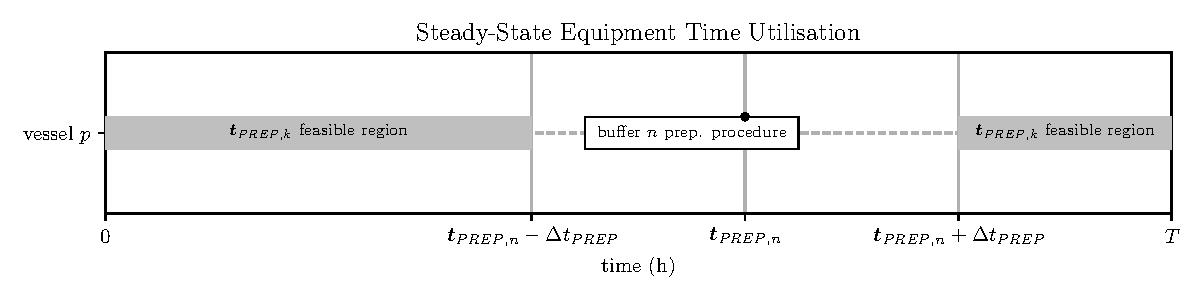
\includegraphics[width=\linewidth]{./figures/sched1.pdf}
    \caption{Example feasible region for buffer $k$ scheduling}
    \label{fig.sched1}
\end{figure}
Imagine, for instance, that a preparation procedure for buffer $n$ occurs in a
given slot such that it is scheduled well away from the cycle time boundaries.
In such a case, we would envisage two feasible time spans wherein a second
preparation procedure (for, e.g.\ buffer $k$) may be scheduled in the same
slot.
In terms of the variables defined in 
\hyperref[SS.schedintro]{Section \ref*{SS.schedintro}}, the situation described
above is represented graphically in 
\hyperref[fig.sched1]{Figure \ref*{fig.sched1}}.
The feasible regions may be summarised as follows:
\begin{equation}
    \begin{split}
        \boldsymbol{t}_{\mathit{PREP},k} \ge \boldsymbol{t}_{\mathit{PREP},n} 
        + \Delta t_{\mathit{PREP}} \quad \text{or} \quad 
        \boldsymbol{t}_{\mathit{PREP},k} \le \boldsymbol{t}_{\mathit{PREP},n}
        - \Delta t_{\mathit{PREP}}\\
        \quad \forall n \in \mathcal{N}, \enspace \forall k \in \mathcal{N}; \;
        k > n
    \end{split}    
    \label{eq.k0}
\end{equation}
Similar to the approach taken in 
\hyperref[SS.absval]{Section \ref*{SS.absval}}, we can convert the \emph{or}
constraints into \emph{and} constraints by defining an additional binary
variable, $\boldsymbol{v}_{nk}$ and using the \emph{big-M} method. In this
case, $\mathbb{M} = 2T$ is sufficient.
\begin{equation}
    \boldsymbol{v}_{nk} \in \left\{ 0, 1 \right\} \quad \forall n \in 
    \mathcal{N}, \enspace \forall k \in \mathcal{N}; \; k > n
    \label{eq.v}
\end{equation}
\begin{equation}
    \begin{split}
        \begin{alignedat}{2}
            2T \boldsymbol{v}_{nk} + \boldsymbol{t}_{\mathit{PREP},k} &{}\ge{}
            \boldsymbol{t}_{\mathit{PREP},n} {}+{} \Delta t_{\mathit{PREP}}\\
            2T \boldsymbol{v}_{nk} + \boldsymbol{t}_{\mathit{PREP},k} &{}\le{}
            \boldsymbol{t}_{\mathit{PREP},n} {}-{} \Delta t_{\mathit{PREP}}
            {}+{} 2T\\
        \end{alignedat}
    \end{split}
    \quad \forall n \in \mathcal{N}, \enspace \forall k \in \mathcal{N}; \;
    k > n
    \label{eq.k1}
\end{equation}
Unfortunately, the above equations do not always hold when the preparation of
one or other of the buffers nears a cycle boundary.
To explain this, \hyperref[fig.sched2]{Figure \ref*{fig.sched2}} (using
\hyperref[fig.sched1]{Figure \ref*{fig.sched1}} as a legend) explores all the
possible cases that must be considered for cyclic scheduling.
\begin{figure}
    \centering
    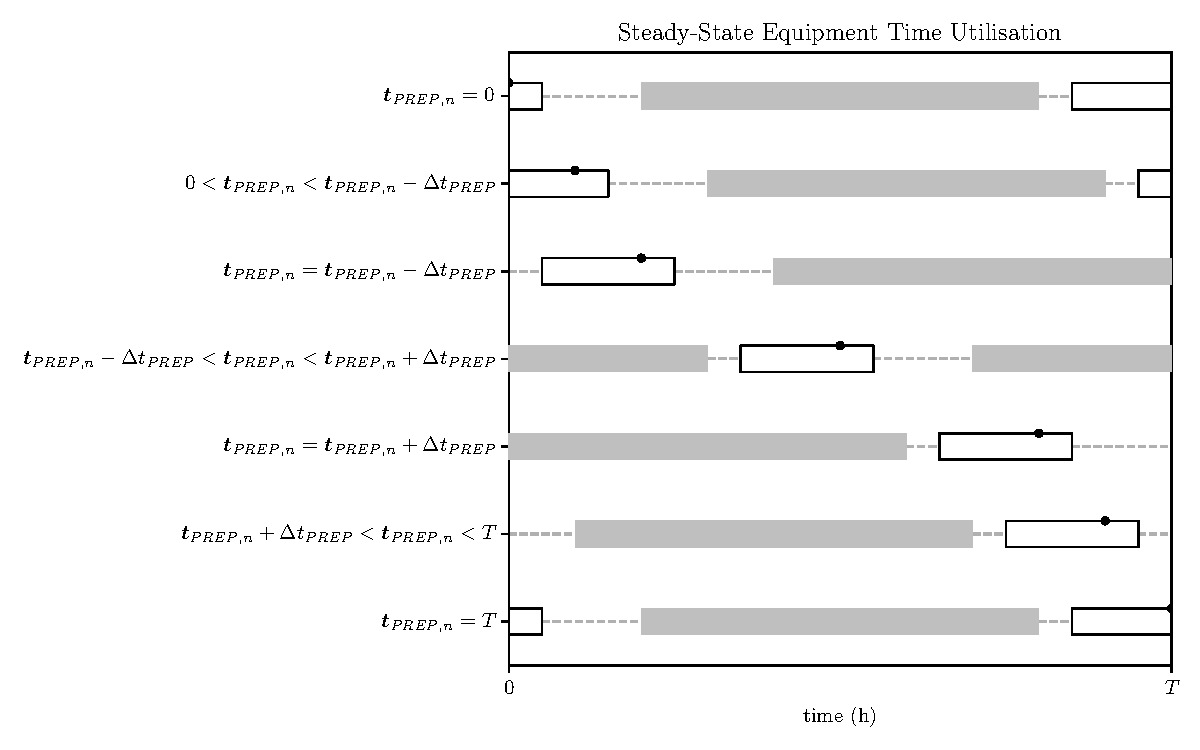
\includegraphics[width=\linewidth]{./figures/sched2.pdf}
    \caption{All feasible region cases for buffer $k$ scheduling}
    \label{fig.sched2}
\end{figure}
Note that the case shown in \hyperref[fig.sched1]{Figure \ref*{fig.sched1}}, 
i.e.\ the case where
$\left( \boldsymbol{t}_{\mathit{PREP},n} - \Delta t_{\mathit{PREP}} \right) \le 
 \boldsymbol{t}_{\mathit{PREP},k} \le
 \left( \boldsymbol{t}_{\mathit{PREP},n} + \Delta t_{\mathit{PREP}} \right)$
is, in fact, the only case where there are two distinct feasible regions.
For all other cases, there is a single feasible region.  We need to be able to
distinguish between these cases.
Note also that the upper and lower bounds of the feasible region cannot always
be found by adding or subtracting a factor of $\Delta t_{\mathit{PREP}}$
to/from $\boldsymbol{t}_{\mathit{PREP},n}$ respectively, as doing so may result
in values outside the single-cycle range in some instances; we need to add some
logic to prevent this.

The lower bound of the feasible region, $\boldsymbol{t}_{\mathit{LOWER},n}$, is
defined as:
\begin{equation}
    \boldsymbol{t}_{\mathit{LOWER},n} = \boldsymbol{t}_{\mathit{PREP},n} +
    \Delta t_{\mathit{PREP}} - T \boldsymbol{r}_{n} \quad \forall n \in
    \mathcal{N}
    \label{eq.lower1}
\end{equation}
where:
\begin{equation}
    0 \le \boldsymbol{t}_{\mathit{LOWER},n} \le T, \quad 
    \boldsymbol{t}_{\mathit{LOWER},n} \in \mathbb{R}, \enspace \forall n \in
    \mathcal{N}
    \label{eq.lower2}
\end{equation}
and:
\begin{equation}
    \boldsymbol{r}_{n} \in \left\{ 0, 1 \right\} \quad \forall n \in
    \mathcal{N}
    \label{eq.r}
\end{equation}
Similarly, the upper bound of the feasible region, 
$\boldsymbol{t}_{\mathit{UPPER},n}$, is defined as:
\begin{equation}
    \boldsymbol{t}_{\mathit{UPPER},n} = \boldsymbol{t}_{\mathit{PREP},n} -
    \Delta t_{\mathit{PREP}} + T \boldsymbol{s}_{n} \quad \forall n \in 
    \mathcal{N}
    \label{eq.upper1}
\end{equation}
where:
\begin{equation}
    0 \le \boldsymbol{t}_{\mathit{UPPER},n} \le T, \quad
    \boldsymbol{t}_{\mathit{LOWER},n} \in \mathbb{R}, \enspace \forall n \in 
    \mathcal{N}
    \label{eq.upper2}
\end{equation}
and:
\begin{equation}
    \boldsymbol{s}_{n} \in \left\{ 0, 1 \right\} \quad \forall n \in
    \mathcal{N}
    \label{eq.s}
\end{equation} 
As was the case with \hyperref[eq.tprep]{equation \ref*{eq.tprep}},
equations \ref{eq.lower1} and \ref{eq.upper1} are equalities and so 
$\boldsymbol{t}_{\mathit{LOWER},n}$ and $\boldsymbol{t}_{\mathit{UPPER},n}$
will be replaced by the right hand sides of equations \ref{eq.lower1} and
\ref{eq.upper1} respectively in the final model to reduce complexity.
The new binary variables, $\boldsymbol{r}_{n}$ and $\boldsymbol{s}_{n}$, are
used to ensure values are kept in the single-cycle range, similar to the
function of $\boldsymbol{q}_{n}$ in
\hyperref[eq.tprep]{equation \ref*{eq.tprep}}:
\begin{equation}
    \begin{split}
        \begin{alignedat}{2}
            T \boldsymbol{r}_{n} \le \Delta t_{\mathit{PREP}}
            + \boldsymbol{t}_{\mathit{PREP},n}&\\
            T \boldsymbol{r}_{n} \ge \Delta t_{\mathit{PREP}}
            + \boldsymbol{t}_{\mathit{PREP},n}& - T\\
            \end{alignedat}
        \quad \forall n \in \mathcal{N}
    \end{split}
    \label{eq.r1}
\end{equation}
\begin{equation}
    \begin{split}
        \begin{alignedat}{2}
            T \boldsymbol{s}_{n} &\ge \Delta t_{\mathit{PREP}}
            - \boldsymbol{t}_{\mathit{PREP},n}\\
            T \boldsymbol{s}_{n} &\le \Delta t_{\mathit{PREP}} 
            -\boldsymbol{t}_{\mathit{PREP},n} + T
        \end{alignedat}
        \quad \forall n \in \mathcal{N}
    \end{split}
    \label{eq.s1}
\end{equation}
Truth tables for equations \ref{eq.r1} and \ref{eq.s1} are given in Tables
\ref{tbl.truthr} and \ref{tbl.truths} respectively.
\begin{table}[h!]
    \centering
    \caption{Truth table for $\boldsymbol{r}_{n}$}
    \label{tbl.truthr}
    \begin{tabular}{c | c c | c}
        $t_{\mathit{USE},n} + \Delta t_{\mathit{PREP}}$
        & $\boldsymbol{r}_{n}^{\left( 1 \right)}$
        & $\boldsymbol{r}_{n}^{\left( 2 \right)}$
        & $\boldsymbol{r}_{n} = \boldsymbol{r}_{n}^{\left( 1 \right)} \land
        \boldsymbol{r}_{n}^{\left( 2 \right)}$\\ \hline
        $< T$ & 0 & $\left\{ 0,1 \right\}$ & 0\\
        $T$ & $\left\{ 0,1 \right\}$ & $\left\{ 0,1 \right\}$
            & $\left\{ 0,1 \right\}$\\
        $>T$ & $\left\{ 0,1 \right\}$ & 1 & 1\\
    \end{tabular}
\end{table}
\begin{table}[h!]
    \centering
    \caption{Truth table for $\boldsymbol{s}_{n}$}
    \label{tbl.truths}
    \begin{tabular}{c | c c | c}
        $t_{\mathit{USE},n} - \Delta t_{\mathit{PREP}}$
        & $\boldsymbol{s}_{n}^{\left( 1 \right)}$
        & $\boldsymbol{s}_{n}^{\left( 2 \right)}$
        & $\boldsymbol{s}_{n} = \boldsymbol{s}_{n}^{\left( 1 \right)} \land
        \boldsymbol{s}_{n}^{\left( 2 \right)}$\\ \hline
        $< 0$ & 1 & $\left\{ 0,1 \right\}$ & 1\\
        0 & $\left\{ 0,1 \right\}$ & $\left\{ 0,1 \right\}$
            & $\left\{ 0,1 \right\}$\\
        $> 0$ & $\left\{ 0,1 \right\}$ & 0 & 0\\
    \end{tabular}
\end{table}

As can be seen from \hyperref[fig.sched2]{Figure \ref*{fig.sched2}},
the feasible region, when contiguous in the single-cycle window,
is bounded below by $\boldsymbol{t}_{\mathit{LOWER},n}$ and above by
$\boldsymbol{t}_{\mathit{UPPER},n}$, giving rise to the following two
constraints:
\begin{equation}
    \begin{split}
        \boldsymbol{t}_{\mathit{PREP},k} 
        \ge \boldsymbol{t}_{\mathit{LOWER},n}\\
        \boldsymbol{t}_{\mathit{PREP},k} 
        \le \boldsymbol{t}_{\mathit{UPPER},n}
    \end{split}
    \quad \forall n \in \mathcal{N}, \enspace \forall k \in \mathcal{N}; \;
    k > n
    \label{eq.k2}
\end{equation}
Recall that constraints on $\boldsymbol{t}_{\mathit{PREP},k}$ were defined in
\hyperref[eq.k1]{equation \ref*{eq.k1}}, for the case where there were two
distinct feasible regions in the cycle.
In \hyperref[eq.k2]{equation \ref*{eq.k2}} above, we have now detailed
constraints on $\boldsymbol{t}_{\mathit{PREP},k}$ for the cases where there is
a single, contiguous feasible region in the cycle.
All that is left to do is to define another binary variable that selects
between these two sets of constraints.
By looking at \hyperref[fig.sched2]{Figure \ref*{fig.sched2}}, it can be seen
that we are only interested in applying the constraints in 
\hyperref[eq.k1]{equation \ref*{eq.k1}} when both
$\boldsymbol{t}_{\mathit{UPPER},n} < \boldsymbol{t}_{\mathit{PREP},n}$ and
$\boldsymbol{t}_{\mathit{LOWER},n} > \boldsymbol{t}_{\mathit{PREP},n}$, i.e.\
when both $\boldsymbol{r}_{n} = 0$ and $\boldsymbol{s}_{n} = 0$.
In all other cases, we wish to apply the constraints in
\hyperref[eq.k2]{equation \ref*{eq.k2}}.
We therefore define a new binary variable, $\boldsymbol{u}_{n}$, where 
$\boldsymbol{u}_{n} = 0$ iff $\boldsymbol{r}_{n} = 0$ and 
$\boldsymbol{s}_{n} = 0$.
\begin{equation}
    \boldsymbol{u}_{n} \in \left\{ 0, 1 \right\} \quad \forall n \in
    \mathcal{N}
    \label{eq.u}
\end{equation}
\begin{equation}
    \begin{split}
        \begin{alignedat}{8}
            \boldsymbol{u}_{n} &\le &&\boldsymbol{r}_{n}
            && {}+{} &&\boldsymbol{s}_{n}\\
            \boldsymbol{u}_{n} &\ge \tfrac{1}{2} &&\boldsymbol{r}_{n}
            && {}+{} \tfrac{1}{2} &&\boldsymbol{s}_{n}\\
        \end{alignedat}
        \quad \forall n \in \mathcal{N}
    \end{split}
    \label{eq.u1}
\end{equation}
A truth table for \hyperref[eq.u1]{equation \ref*{eq.u1}} is given in 
\hyperref[tbl.truthu]{Table \ref*{tbl.truthu}}.
\begin{table}[h!]
    \centering
    \caption{Truth table for $\boldsymbol{u}_{n}$}
    \label{tbl.truthu}
    \begin{tabular}{c c | c c | c}
        $\boldsymbol{r}_{n}$ & $\boldsymbol{s}_{n}$ &
        $\boldsymbol{u}_{n}^{\left( 1 \right)}$ &
        $\boldsymbol{u}_{n}^{\left( 2 \right)}$ &
        $\boldsymbol{u}_{n} = \boldsymbol{u}_{n}^{\left( 1 \right)}
            \land \boldsymbol{u}_{n}^{\left( 2 \right)}
        $\\ \hline
        0 & 0 & 0 & $\left\{ 0,1 \right\}$ & 0\\
        0 & 1 & $\left\{ 0,1 \right\}$ & 1 & 1\\
        1 & 0 & $\left\{ 0,1 \right\}$ & 1 & 1\\
        1 & 1 & $\left\{ 0,1 \right\}$ & 1 & 1\\
    \end{tabular}
\end{table}
With the definition of $\boldsymbol{u}_{n}$, a unified set of inequalities can
be written which describe the scheduling of buffers prepared in the same slot.
Once again, the \emph{big-M} method is employed, with $\mathbb{M} = 2T$.
\begin{equation}
    \begin{split}
        \begin{alignedat}{10}
            \boldsymbol{t}_{\mathit{PREP},k}
            &\le \boldsymbol{t}_{\mathit{PREP},n}
            - \Delta t_{\mathit{PREP}} {}+{} & 2T &\boldsymbol{u}_{n}
            {}-{} & 2T &\boldsymbol{v}_{nk} & {}+{} 2T&\\
            \boldsymbol{t}_{\mathit{PREP},k}
            &\ge \boldsymbol{t}_{\mathit{PREP},n}
            + \Delta t_{\mathit{PREP}} {}-{} & 2T &\boldsymbol{u}_{n}
            {}-{} & 2T &\boldsymbol{v}_{nk}&\\
            \boldsymbol{t}_{\mathit{PREP},k}
            &\le \boldsymbol{t}_{\mathit{PREP},n}
            - \Delta t_{\mathit{PREP}} {}-{} & 2T &\boldsymbol{u}_{n}
            {}+{} & T &\boldsymbol{r}_{n} & {}+{} 2T&\\
            \boldsymbol{t}_{\mathit{PREP},k}
            &\ge \boldsymbol{t}_{\mathit{PREP},n}
            + \Delta t_{\mathit{PREP}} {}+{} & 2T &\boldsymbol{u}_{n}
            {}-{} & T &\boldsymbol{s}_{n} & {}-{} 2T&\\
            &\forall n \in \mathcal{N}, \enspace \forall k \in \mathcal{N}; \;
            k > n
            \end{alignedat}            
    \end{split}
    \label{eq.k4}
\end{equation}

\subsection{Preparation Scheduling}\label{SS.prepsched}
The constraints in \hyperref[eq.k4]{equation \ref*{eq.k4}} are only valid for
the case where buffers $n$ and $k$ are prepared in the same slot.
Recall that we defined a variable, $\boldsymbol{a}_{nk}$, which indicated if
this is the case.
Accordingly, the final preparation scheduling constraint is a modification of
\hyperref[eq.k4]{equation \ref*{eq.k4}} which uses the \emph{big-M} method,
with $\mathbb{M} = 2T$, to disable all of the constraints when
$\boldsymbol{a}_{nk} = 0$.
The final preparation constraint is given in equation
\hyperref[eq.k5]{equation \ref*{eq.k5}} below. 
\begin{equation}
    \begin{split}
        \begin{alignedat}{14}
            \boldsymbol{t}_{\mathit{PREP},k}
            &\le \boldsymbol{t}_{\mathit{PREP},n}
            - \Delta t_{\mathit{PREP}} {}-{} & 2T &\boldsymbol{a}_{nk}
            {}+{} & 2T &\boldsymbol{u}_{n}
            {}-{} & 2T &\boldsymbol{v}_{nk} & {}+{} 4T&\\
            \boldsymbol{t}_{\mathit{PREP},k}
            &\ge \boldsymbol{t}_{\mathit{PREP},n}
            + \Delta t_{\mathit{PREP}} {}+{} & 2T &\boldsymbol{a}_{nk}
            {}-{} & 2T &\boldsymbol{u}_{n}
            {}-{} & 2T &\boldsymbol{v}_{nk} & {}-{} 2T&\\
            \boldsymbol{t}_{\mathit{PREP},k}
            &\le \boldsymbol{t}_{\mathit{PREP},n}
            - \Delta t_{\mathit{PREP}} {}-{} & 2T &\boldsymbol{a}_{nk}
            {}-{} & 2T &\boldsymbol{u}_{n}
            {}+{} & T &\boldsymbol{r}_{n} & {}+{} 4T&\\
            \boldsymbol{t}_{\mathit{PREP},k}
            &\ge \boldsymbol{t}_{\mathit{PREP},n}
            + \Delta t_{\mathit{PREP}} {}+{} & 2T &\boldsymbol{a}_{nk}
            {}+{} & 2T &\boldsymbol{u}_{n}
            {}-{} & T &\boldsymbol{s}_{n} & {}-{} 4T&\\
            &\forall n \in \mathcal{N}, \enspace \forall k \in \mathcal{N}; \;
            k > n
            \end{alignedat}            
    \end{split}
    \label{eq.k5}
\end{equation}

A truth table for \hyperref[eq.k5]{equation \ref*{eq.k5}} is given in
\hyperref[tbl.truthsched]{Table \ref*{tbl.truthsched}}, with `$\ast$' denoting
the binary set, $\left\{0,1\right\}$.
Recall also that \hyperref[eq.tprep1]{equation \ref*{eq.tprep1}} implies
$0 \le \boldsymbol{t}_{\mathit{PREP},k} \le T$, so we do not need
\hyperref[eq.k5]{equation \ref*{eq.k5}} to duplicate that constraint.
\begin{table}[h!]
    \centering
    \caption{Truth table for equation \ref{eq.k5}}
    \label{tbl.truthsched}
    \begin{tabular}{c c c c c | c}
        $\boldsymbol{a}_{nk}$ & $\boldsymbol{u}_{n}$ & $\boldsymbol{v}_{n}$
        & $\boldsymbol{r}_{n}$ & $\boldsymbol{s}_{n}$
        & $\boldsymbol{t}_{\mathit{PREP},k} = \bullet$\\\hline
        0 & $\ast$ & $\ast$ & $\ast$ & $\ast$ 
        & (no active scheduling constraints)\\
        1 & 0 & 0 & $\ast$ & $\ast$
        & $\boldsymbol{t}_{\mathit{PREP},n} + \Delta t_{\mathit{PREP}} \le
            \bullet $\\
        1 & 0 & 1 & $\ast$ & $\ast$ 
        & $\bullet \le \boldsymbol{t}_{\mathit{PREP},n} 
           - \Delta t_{\mathit{PREP}}$\\
        1 & 1 & $\ast$ & 0 & 0 
        & $\boldsymbol{t}_{\mathit{PREP},n} + \Delta t_{\mathit{PREP}}
           \le \bullet \le \boldsymbol{t}_{\mathit{PREP},n} 
           - \Delta t_{\mathit{PREP}}$\\
        1 & 1 & $\ast$ & 0 & 1 
        & $\boldsymbol{t}_{\mathit{PREP},n} + \Delta t_{\mathit{PREP}} - T
           \le \bullet \le \boldsymbol{t}_{\mathit{PREP},n}
           - \Delta t_{\mathit{PREP}}$\\
        1 & 1 & $\ast$ & 1 & 0 
        & $\boldsymbol{t}_{\mathit{PREP},n} + \Delta t_{\mathit{PREP}}
           \le \bullet \le \boldsymbol{t}_{\mathit{PREP},n}
           - \Delta t_{\mathit{PREP}} + T$\\
        1 & 1 & $\ast$ & 1 & 1 
        & $\boldsymbol{t}_{\mathit{PREP},n} + \Delta t_{\mathit{PREP}} - T
           \le \bullet \le \boldsymbol{t}_{\mathit{PREP},n}
           - \Delta t_{\mathit{PREP}} + T$\\
    \end{tabular}
\end{table}


\subsection{Complete Model Summary}\label{SS.completesummary}

The complete model is summarised below.
The constraint equations have been rearranged so that variables are on the left
hand side and constants are on the right. 

Minimise:
\begin{equation}
    \boldsymbol{Z} = \sum_{m \in \mathcal{M}} \sum_{p \in \mathcal{P}} c_m
    \boldsymbol{y}_{mp}
    \tag{\ref{eq.objfn}}
\end{equation}
Subject to:
\begin{equation}
    \sum_{p \in \mathcal{P}} \boldsymbol{x}_{np} = 1 \quad \forall n \in 
    \mathcal{N}
    \tag{\ref{eq.constr1}}
\end{equation}
\begin{equation}
    \sum_{m \in \mathcal{M}} \boldsymbol{y}_{mp} \le 1 \quad \forall p \in 
    \mathcal{P}
    \tag{\ref{eq.constr2}}
\end{equation}
\begin{equation}
    U_{n} \boldsymbol{x}_{np} - \sum_{m \in \mathcal{M}} V_{m} 
    \boldsymbol{y}_{mp} \le 0 \quad \forall n \in \mathcal{N}, \enspace 
    \forall p \in \mathcal{P}
    \tag{\ref{eq.constr3a}}
\end{equation}
\begin{equation}
    V_{\mathit{MAX}} \boldsymbol{x}_{np} + f_{\mathit{MINFILL}} 
    \sum_{m \in \mathcal{M}} V_{m} \boldsymbol{y}_{mp} \le U_{n}
    + V_{\mathit{MAX}} \quad \forall n \in \mathcal{N}, \enspace \forall p \in
    \mathcal{P}
    \tag{\ref{eq.constr3b}}
\end{equation}
\begin{equation}
    \Delta t_{\mathit{PREP}} \sum_{n \in \mathcal{N}} \boldsymbol{x}_{np} \le
    f_{\mathit{UTIL}} T \quad \forall p \in \mathcal{P}
    \tag{\ref{eq.constr4}}
\end{equation}
%new equations
\begin{equation}
    \begin{aligned}
        \boldsymbol{z}_{n} \le T - \Delta t_{\mathit{HOLD,PRE}}
        - \Delta t_{\mathit{TRANSFER}} - \Delta t_{\mathit{USE},n}
        - \Delta t_{\mathit{HOLD,POST}}\\
        \quad \forall n \in \mathcal{N}
    \end{aligned}
    \tag{\ref{eq.z1}}
\end{equation}
\begin{equation}
    \begin{split}
        \begin{alignedat}{11}
            2&\boldsymbol{w}_{nkp} {}-{} &&\boldsymbol{x}_{np}
            {}-{} && \boldsymbol{x}_{kp} {}&&\le{} &{}-{} 2\\
            &\boldsymbol{w}_{nkp} {}-{} &&\boldsymbol{x}_{np}
            {}-{} && \boldsymbol{x}_{kp} {}&&\ge{} &{}-{} 1\\
        \end{alignedat}
    \end{split}
    \quad
    \begin{split}
        \forall n \in \mathcal{N}, \enspace \forall k \in \mathcal{N}; \; 
        k > n, \enspace \forall p \in \mathcal{P}
    \end{split}
    \tag{\ref{eq.w1}}
\end{equation}
\begin{equation}
    \begin{split}
        \begin{alignedat}{2}
            T \boldsymbol{q}_{n} - \boldsymbol{z}_{n} &\ge
            - t_{\mathit{USE},n}\\
            T \boldsymbol{q}_{n} - \boldsymbol{z}_{n} &\le
            - t_{\mathit{USE},n} + T\\
        \end{alignedat}
    \end{split}
    \quad \forall n \in \mathcal{N}
    \tag{\ref{eq.q1}}
\end{equation}
\begin{equation}
    \begin{split}
        \begin{alignedat}{2}
            -T \boldsymbol{q}_{n} + T \boldsymbol{r}_{n} + \boldsymbol{z}_{n}
            &\le t_{\mathit{USE},n} + \Delta t_{\mathit{PREP}}\\
            -T \boldsymbol{q}_{n} + T \boldsymbol{r}_{n} + \boldsymbol{z}_{n}
            &\ge t_{\mathit{USE},n} + \Delta t_{\mathit{PREP}} - T\\
            \end{alignedat}
        \quad \forall n \in \mathcal{N}
    \end{split}
    \label{eq.r2}
\end{equation}
\begin{equation}
    \begin{split}
        \begin{alignedat}{2}
            T \boldsymbol{q}_{n} + T \boldsymbol{s}_{n} - \boldsymbol{z}_{n}
            &\le -t_{\mathit{USE},n} + \Delta t_{\mathit{PREP}}\\
            T \boldsymbol{q}_{n} + T \boldsymbol{s}_{n} - \boldsymbol{z}_{n}
            &\ge -t_{\mathit{USE},n} + \Delta t_{\mathit{PREP}} + T\\
            \end{alignedat}
        \quad \forall n \in \mathcal{N}
    \end{split}
    \label{eq.s2}
\end{equation}
\begin{equation}
    \begin{split}
        \begin{alignedat}{8}
            &&\boldsymbol{r}_{n} && {}+{} &&\boldsymbol{s}_{n} && {}-{} 
            &&\boldsymbol{u}_{n} &\ge 0\\
            &&\boldsymbol{r}_{n} && {}+{} &&\boldsymbol{s}_{n} && {}-{} 
            &2&\boldsymbol{u}_{n} &\le 0\\
        \end{alignedat}
        \quad \forall n \in \mathcal{N}
    \end{split}
    \tag{\ref{eq.u1}}
\end{equation}
\begin{equation}
    \begin{split}
        \begin{aligned}
            T \boldsymbol{q}_{k} - T \boldsymbol{q}_{n} + 2T \boldsymbol{u}_{n} 
            + 2T \boldsymbol{v}_{nk} - 2T \sum_{p \in \mathcal{P}}
            \boldsymbol{w}_{nkp} - \boldsymbol{z}_{k} + \boldsymbol{z}_{n}\\
            \ge t_{\mathit{USE},n} - t_{\mathit{USE},k}
            + \Delta t_{\mathit{PREP}} - 2T
        \end{aligned}\\
        \begin{aligned}
            T \boldsymbol{q}_{k} - T \boldsymbol{q}_{n} - 2T \boldsymbol{u}_{n} 
            + 2T \boldsymbol{v}_{nk} + 2T \sum_{p \in \mathcal{P}}
            \boldsymbol{w}_{nkp} - \boldsymbol{z}_{k} + \boldsymbol{z}_{n}\\
            \ge t_{\mathit{USE},n} - t_{\mathit{USE},k}
            - \Delta t_{\mathit{PREP}} + 4T
        \end{aligned}\\
        \begin{aligned}
            T \boldsymbol{q}_{k} - T \boldsymbol{q}_{n} - T \boldsymbol{r}_{n}
            + 2T \boldsymbol{u}_{n} + 2T \sum_{p \in \mathcal{P}}
            \boldsymbol{w}_{nkp} - \boldsymbol{z}_{k} + \boldsymbol{z}_{n}\\
            \ge t_{\mathit{USE},n} - t_{\mathit{USE},k}
            - \Delta t_{\mathit{PREP}} + 4T
        \end{aligned}\\
        \begin{aligned}
            T \boldsymbol{q}_{k} - T \boldsymbol{q}_{n} + T \boldsymbol{s}_{n}
            - 2T \boldsymbol{u}_{n} - 2T \sum_{p \in \mathcal{P}}
            \boldsymbol{w}_{nkp} - \boldsymbol{z}_{k} + \boldsymbol{z}_{n}\\
            \ge t_{\mathit{USE},n} - t_{\mathit{USE},k}
            + \Delta t_{\mathit{PREP}} - 4T
        \end{aligned}\\
        \begin{aligned}
            \forall n \in \mathcal{N}, \enspace \forall k \in \mathcal{N}; \;
            k > n
        \end{aligned}\\
    \end{split}
    \label{eq.k6}
\end{equation}
Where:
\begin{equation}
    \boldsymbol{q}_{n} \in \left\{0, 1\right\} \quad \forall n \in \mathcal{N}
    \tag{\ref{eq.q}}
\end{equation}
\begin{equation}
    \boldsymbol{r}_{n} \in \left\{ 0, 1 \right\} \quad \forall n \in
    \mathcal{N}
    \tag{\ref{eq.r}}
\end{equation}
\begin{equation}
    \boldsymbol{s}_{n} \in \left\{ 0, 1 \right\} \quad \forall n \in
    \mathcal{N}
    \tag{\ref{eq.s}}
\end{equation} 
\begin{equation}
    \boldsymbol{u}_{n} \in \left\{ 0, 1 \right\} \quad \forall n \in
    \mathcal{N}
    \tag{\ref{eq.u}}
\end{equation}
\begin{equation}
    \boldsymbol{v}_{nk} \in \left\{ 0, 1 \right\} \quad \forall n \in
    \mathcal{N}, \enspace \forall k \in \mathcal{N}; \; k > n
    \tag{\ref{eq.v}}
\end{equation}
\begin{equation}
    \boldsymbol{w}_{nkp} \in \left\{ 0, 1 \right\} \quad \forall n \in
    \mathcal{N}, \enspace \forall k \in \mathcal{N}; \; k > n, \enspace \forall
    p \in \mathcal{P}
    \tag{\ref{eq.w}}
\end{equation}
\begin{equation}
    \boldsymbol{x}_{np} \in \left\{ 0, 1 \right\} \quad \forall n \in
    \mathcal{N}, \enspace \forall p \in \mathcal{P}
    \tag{\ref{eq.x}}
\end{equation}
\begin{equation}
    \boldsymbol{y}_{mp} \in \left\{ 0, 1 \right\} \quad \forall m \in
    \mathcal{M}, \enspace \forall p \in \mathcal{P}
    \tag{\ref{eq.y}}
\end{equation}
\begin{equation}
    \Delta t_{\mathit{HOLD,MIN}} \le \boldsymbol{z}_{n} \le 
    \Delta t_{\mathit{HOLD,MAX}}; \quad
    \boldsymbol{z}_{n} \in \mathbb{R} \quad \forall n \in \mathcal{N}
    \tag{\ref{eq.z}}
\end{equation}

Note that variables $\boldsymbol{a}_{nk}$, $\boldsymbol{t}_{\mathit{PREP},n}$,
$\boldsymbol{t}_{\mathit{PREP},k}$, $\boldsymbol{t}_{\mathit{LOWER},n}$ and
$\boldsymbol{t}_{\mathit{UPPER},n}$ are not required in the model. Values for
these variables can be obtained, post solution, by applying equations
\ref{eq.a1}, \ref{eq.tprep}, \ref{eq.tprep} (replacing $n$ with $k$),
\ref{eq.lower1} and \ref{eq.upper1} respectively.

\section{Further Optimisation}\label{S.secondary}

\subsection{Goal programming}\label{SS.goal}
The complete model summarised in 
\hyperref[SS.completesummary]{Section \ref*{SS.completesummary}} may be solved
to give the required number of vessels that correspond to the minimum cost.
As was alluded to in \hyperref[S.outputdata]{Section \ref*{S.outputdata}},
there may be many possible feasible solutions that correspond to this minimum
cost and would yield the same set of vessels (though the selected preparation
vessels may not necessarily be used to prepare the same buffers).
Thus, there may be many ways to represent an optimal process schedule.

If, for example, the data described in
\hyperref[C.data]{Chapter \ref*{C.data}} were used as an input to the complete
model, an \emph{equipment time utilisation} plot (see
\hyperref[S.outputdata]{Section \ref*{S.outputdata}}) for the feasible optimal
schedule (such as that shown in 
\hyperref[fig.primary]{Figure \ref*{fig.primary}})
may be generated.
\begin{figure}
    \centering
    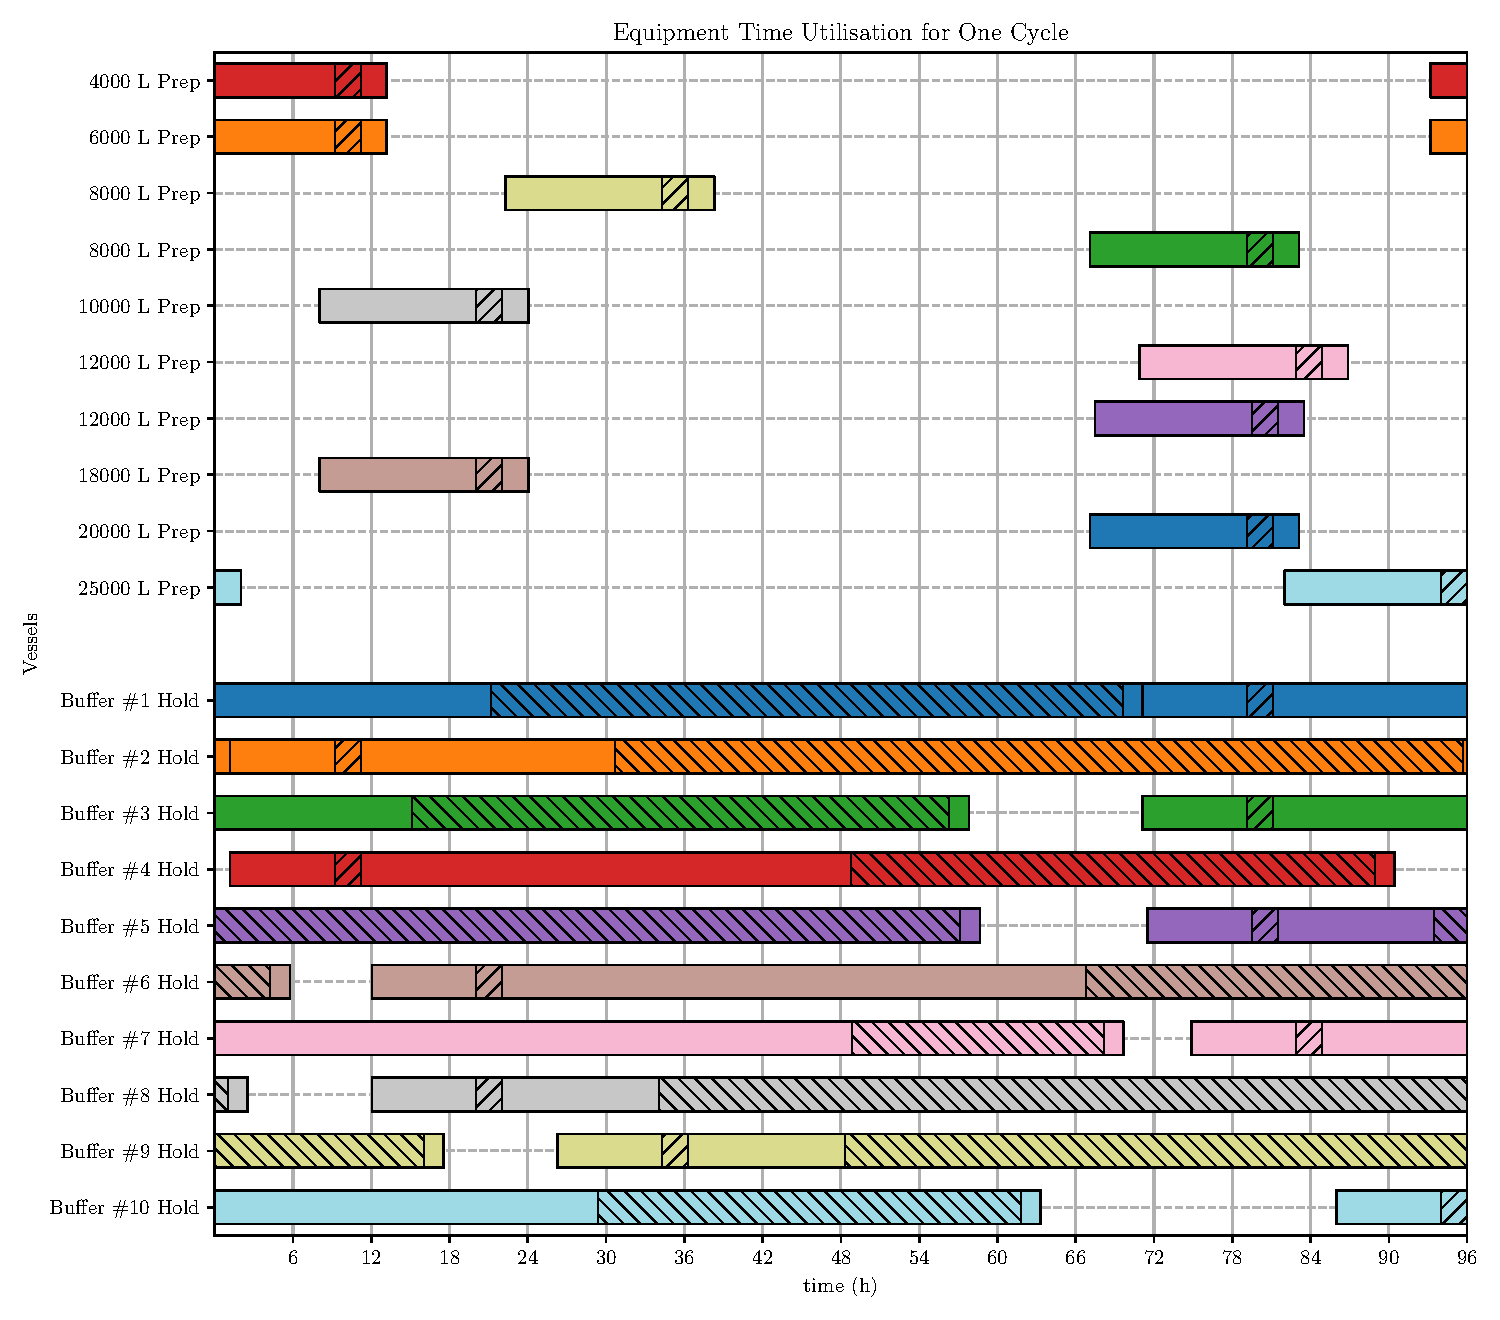
\includegraphics[width=\linewidth]{./figures/plot1.pdf}
    \caption{Random example -- primary objective (note that buffers are
        individually coloured; each buffer has its own hold vessel, from which
        its colour may be determined)}
    \label{fig.primary}
\end{figure}

Note that the solution requires four vessels, with sizes
\SI{2000}{\litre}, \SI{8000}{\litre}, \SI{25000}{\litre} and \SI{30000}{\litre}
respectively.  
Recall that one of our decision variables is $\boldsymbol{z}_{n}$, the buffer
hold duration.
In \hyperref[fig.primary]{Figure \ref*{fig.primary}}, we can see that Buffer
\#2 is scheduled such that its hold procedure is bottlenecked, i.e.\ the start
of the hold procedure for a given batch coincides precisely with the end of the
hold procedure for the previous batch.
For this buffer, it can also be seen that there exists some free time after
its preparation procedure.

Delaying the preparation of Buffer \#2 by e.g.\ three hours would
also give an optimal solution, with the vessel selection unchanged and would
prevent the hold procedure for Buffer \#2 from being bottlenecked.
There exists sufficient free time in the \SI{8000}{\litre} vessel to do this.
Note that delaying a preparation by some amount $\delta$ is equivalent to 
reducing $\boldsymbol{z}_{n}$ by $\delta$.
Recall also that $\boldsymbol{z}_{n}$ has a lower bound, 
$\Delta t_{\mathit{HOLD,MIN}}$.

In terms of visualising a realistic schedule, it is desirable to minimise the
hold durations, i.e.\ we wish to define a new objective function, to be
minimised:
\begin{equation}
    \boldsymbol{Y} = \sum_{n \in \mathcal{N}} \boldsymbol{z}_{n}
    \label{eq.objfn2}
\end{equation}
Note that we want to maintain the original optimum objective function value,
i.e.\ we define:
\begin{equation}
    Z^{\prime} = \min \boldsymbol{Z}
    \label{eq.Zprime}
\end{equation}
In \hyperref[eq.Zprime]{equation \ref*{eq.Zprime}}, $Z^{\prime}$ is the optimal objective function value
obtained by solving the complete model.
Note that $Z^{\prime}$ is not in bold, as it is treated as a constant parameter
in our second-pass model.
The complete model is then re-run with the original objective function replaced
by the new objective, \hyperref[eq.objfn2]{equation \ref*{eq.objfn2}}, with the
following constraint added:
\begin{equation}
    \sum_{m \in \mathcal{M}} \sum_{p \in \mathcal{P}} c_m \boldsymbol{y}_{mp}
    = Z^{\prime}
    \label{eq.constr10}
\end{equation}
\begin{figure}
    \centering
    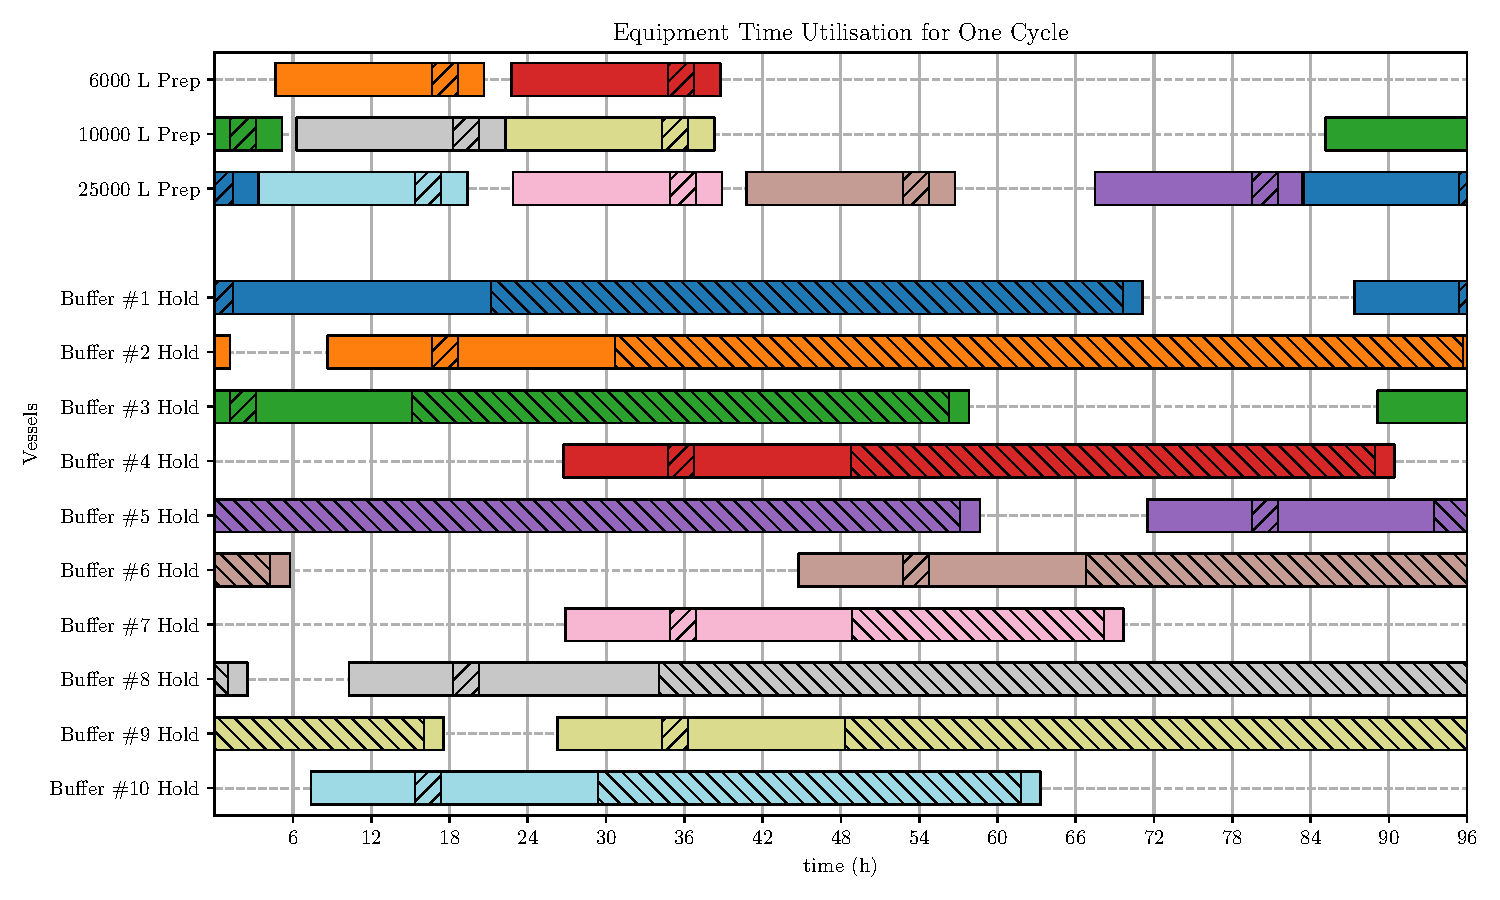
\includegraphics[width=\linewidth]{./figures/plot2.pdf}
    \caption{Random example -- secondary objective}
    \label{fig.secondary}
\end{figure}

Implementing the secondary goal programming model on the same data-set yields
the plot shown in \hyperref[fig.secondary]{Figure \ref*{fig.secondary}}.
Note that the buffer hold procedure for Buffer \#2 is no longer bottlenecked.
We can also see that the hold times for Buffers \#1, \#6, \#7 and \#12 have
all decreased, but the hold time for buffer \#4 has increased.
Overall, there has been a reduction in total hold time, which was our aim.
Note also that, although the same preparation vessels are selected (i.e.\ the
same minimal cost is obtained), some buffers are now prepared in different
vessels to those originally assigned.
For example, in the original result, Buffers \#1 and \#6 were prepared in the
\SI{25000}{\litre} vessel and with the secondary goal added, they are now
prepared in the \SI{30000}{\litre} vessel.
Conversely, preparation of Buffer \#7 shifts from the \SI{30000}{\litre} vessel
to the \SI{25000}{\litre} vessel.

\subsection{Secondary Model Summary}\label{SS.model2summary}

The secondary model is summarised below:

Minimise:
\begin{equation}
    \boldsymbol{Y} = \sum_{n \in \mathcal{N}} \boldsymbol{z}_{n}
    \tag{\ref{eq.objfn2}}
\end{equation}
Subject to:
\begin{equation}
    \sum_{p \in \mathcal{P}} \boldsymbol{x}_{np} = 1 \quad \forall n \in
    \mathcal{N}
    \tag{\ref{eq.constr1}}
\end{equation}
\begin{equation}
    \sum_{m \in \mathcal{M}} \boldsymbol{y}_{mp} \le 1 \quad \forall p \in
    \mathcal{P}
    \tag{\ref{eq.constr2}}
\end{equation}
\begin{equation}
    U_{n} \boldsymbol{x}_{np} - \sum_{m \in \mathcal{M}} V_{m}
    \boldsymbol{y}_{mp} \le 0 \quad \forall n \in \mathcal{N}, \enspace \forall
    p \in \mathcal{P}
    \tag{\ref{eq.constr3a}}
\end{equation}
\begin{equation}
    V_{\mathit{MAX}} \boldsymbol{x}_{np} + f_{\mathit{MINFILL}} \sum_{m \in 
    \mathcal{M}} V_{m} \boldsymbol{y}_{mp} \le U_{n} + V_{\mathit{MAX}} \quad
    \forall n \in \mathcal{N}, \enspace \forall p \in \mathcal{P}
    \tag{\ref{eq.constr3b}}
\end{equation}
\begin{equation}
    \Delta t_{\mathit{PREP}} \sum_{n \in \mathcal{N}} \boldsymbol{x}_{np} \le
    f_{\mathit{UTIL}} T \quad \forall p \in \mathcal{P}
    \tag{\ref{eq.constr4}}
\end{equation}
\begin{equation}
    \begin{aligned}
        \boldsymbol{z}_{n} \le T - \Delta t_{\mathit{HOLD,PRE}}
        - \Delta t_{\mathit{TRANSFER}} - \Delta t_{\mathit{USE},n}
        - \Delta t_{\mathit{HOLD,POST}}\\
        \quad \forall n \in \mathcal{N}
    \end{aligned}
    \tag{\ref{eq.z1}}
\end{equation}
\begin{equation}
    \begin{split}
        \begin{alignedat}{11}
            2&\boldsymbol{w}_{nkp} {}-{} &&\boldsymbol{x}_{np}
            {}-{} && \boldsymbol{x}_{kp} {}&&\le{} &{}-{} 2\\
            &\boldsymbol{w}_{nkp} {}-{} &&\boldsymbol{x}_{np}
            {}-{} && \boldsymbol{x}_{kp} {}&&\ge{} &{}-{} 1\\
        \end{alignedat}
    \end{split}
    \quad
    \begin{split}
        \forall n \in \mathcal{N}, \enspace \forall k \in \mathcal{N}; \;
        k > n, \enspace \forall p \in \mathcal{P}
    \end{split}
    \tag{\ref{eq.w1}}
\end{equation}
\begin{equation}
    \begin{split}
        \begin{alignedat}{2}
            T \boldsymbol{q}_{n} - \boldsymbol{z}_{n} &\ge
            - t_{\mathit{USE},n}\\
            T \boldsymbol{q}_{n} - \boldsymbol{z}_{n} &\le
            - t_{\mathit{USE},n} + T\\
        \end{alignedat}
    \end{split}
    \quad \forall n \in \mathcal{N}
    \tag{\ref{eq.q1}}
\end{equation}
\begin{equation}
    \begin{split}
        \begin{alignedat}{2}
            -T \boldsymbol{q}_{n} + T \boldsymbol{r}_{n} + \boldsymbol{z}_{n}
            &\le t_{\mathit{USE},n} + \Delta t_{\mathit{PREP}}\\
            -T \boldsymbol{q}_{n} + T \boldsymbol{r}_{n} + \boldsymbol{z}_{n}
            &\ge t_{\mathit{USE},n} + \Delta t_{\mathit{PREP}} - T\\
            \end{alignedat}
        \quad \forall n \in \mathcal{N}
    \end{split}
    \tag{\ref{eq.r2}}
\end{equation}
\begin{equation}
    \begin{split}
        \begin{alignedat}{2}
            T \boldsymbol{q}_{n} + T \boldsymbol{s}_{n} - \boldsymbol{z}_{n}
            &\le -t_{\mathit{USE},n} + \Delta t_{\mathit{PREP}}\\
            T \boldsymbol{q}_{n} + T \boldsymbol{s}_{n} - \boldsymbol{z}_{n}
            &\ge -t_{\mathit{USE},n} + \Delta t_{\mathit{PREP}} + T\\
            \end{alignedat}
        \quad \forall n \in \mathcal{N}
    \end{split}
    \tag{\ref{eq.s2}}
\end{equation}
\begin{equation}
    \begin{split}
        \begin{alignedat}{8}
            &&\boldsymbol{r}_{n} && {}+{} &&\boldsymbol{s}_{n} && {}-{} 
            &&\boldsymbol{u}_{n} &\ge 0\\
            &&\boldsymbol{r}_{n} && {}+{} &&\boldsymbol{s}_{n} && {}-{} 
            &2&\boldsymbol{u}_{n} &\le 0\\
        \end{alignedat}
        \quad \forall n \in \mathcal{N}
    \end{split}
    \tag{\ref{eq.u1}}
\end{equation}
\begin{equation}
    \begin{split}
        \begin{aligned}
            T \boldsymbol{q}_{k} - T \boldsymbol{q}_{n} + 2T \boldsymbol{u}_{n} 
            + 2T \boldsymbol{v}_{nk} - 2T \sum_{p \in P} \boldsymbol{w}_{nkp} 
            - \boldsymbol{z}_{k} + \boldsymbol{z}_{n}\\
            \ge t_{\mathit{USE},n} - t_{\mathit{USE},k}
            + \Delta t_{\mathit{PREP}} - 2T
        \end{aligned}\\
        \begin{aligned}
            T \boldsymbol{q}_{k} - T \boldsymbol{q}_{n} - 2T \boldsymbol{u}_{n} 
            + 2T \boldsymbol{v}_{nk} + 2T \sum_{p \in P} \boldsymbol{w}_{nkp} 
            - \boldsymbol{z}_{k} + \boldsymbol{z}_{n}\\
            \ge t_{\mathit{USE},n} - t_{\mathit{USE},k}
            - \Delta t_{\mathit{PREP}} + 4T
        \end{aligned}\\
        \begin{aligned}
            T \boldsymbol{q}_{k} - T \boldsymbol{q}_{n} - T \boldsymbol{r}_{n}
            + 2T \boldsymbol{u}_{n} + 2T \sum_{p \in P} \boldsymbol{w}_{nkp} 
            - \boldsymbol{z}_{k} + \boldsymbol{z}_{n}\\
            \ge t_{\mathit{USE},n} - t_{\mathit{USE},k}
            - \Delta t_{\mathit{PREP}} + 4T
        \end{aligned}\\
        \begin{aligned}
            T \boldsymbol{q}_{k} - T \boldsymbol{q}_{n} + T \boldsymbol{s}_{n}
            - 2T \boldsymbol{u}_{n} - 2T \sum_{p \in P} \boldsymbol{w}_{nkp} 
            - \boldsymbol{z}_{k} + \boldsymbol{z}_{n}\\
            \ge t_{\mathit{USE},n} - t_{\mathit{USE},k}
            + \Delta t_{\mathit{PREP}} - 4T
        \end{aligned}\\
        \begin{aligned}
            \forall n \in \mathcal{N}, \enspace \forall k \in \mathcal{N}; \;
            k > n
        \end{aligned}\\
    \end{split}
    \tag{\ref{eq.k6}}
\end{equation}
\begin{equation}
    \sum_{m \in \mathcal{M}} \sum_{p \in \mathcal{P}} c_m 
    \boldsymbol{y}_{mp} = Z^{\prime}
    \tag{\ref{eq.constr10}}
\end{equation}
Where:
\begin{equation}
    \boldsymbol{q}_{n} \in \left\{0, 1\right\} \quad \forall n \in \mathcal{N}
    \tag{\ref{eq.q}}
\end{equation}
\begin{equation}
    \boldsymbol{r}_{n} \in \left\{ 0, 1 \right\} \quad \forall n \in
    \mathcal{N}
    \tag{\ref{eq.r}}
\end{equation}
\begin{equation}
    \boldsymbol{s}_{n} \in \left\{ 0, 1 \right\} \quad \forall n \in
    \mathcal{N}
    \tag{\ref{eq.s}}
\end{equation} 
\begin{equation}
    \boldsymbol{u}_{n} \in \left\{ 0, 1 \right\} \quad \forall n \in
    \mathcal{N}
    \tag{\ref{eq.u}}
\end{equation}
\begin{equation}
    \boldsymbol{v}_{nk} \in \left\{ 0, 1 \right\} \quad \forall n \in
    \mathcal{N}, \enspace \forall k \in \mathcal{N}; \; k > n
    \tag{\ref{eq.v}}
\end{equation}
\begin{equation}
    \boldsymbol{w}_{nkp} \in \left\{ 0, 1 \right\} \quad \forall n \in 
    \mathcal{N}, \enspace \forall k \in \mathcal{N}; \; k > n, \enspace \forall
    p \in \mathcal{P}
    \tag{\ref{eq.w}}
\end{equation}
\begin{equation}
    \boldsymbol{x}_{np} \in \left\{ 0, 1 \right\} \quad \forall n \in
    \mathcal{N}, \enspace \forall p \in \mathcal{P}
    \tag{\ref{eq.x}}
\end{equation}
\begin{equation}
    \boldsymbol{y}_{mp} \in \left\{ 0, 1 \right\} \quad \forall m \in
    \mathcal{M}, \enspace \forall p \in \mathcal{P}
    \tag{\ref{eq.y}}
\end{equation}
\begin{equation}
    \Delta t_{\mathit{HOLD,MIN}} \le \boldsymbol{z}_{n} \le 
    \Delta t_{\mathit{HOLD,MAX}}; \quad
    \boldsymbol{z}_{n} \in \mathbb{R} \quad \forall n \in \mathcal{N}
    \tag{\ref{eq.z}}
\end{equation}

\section{Implementation}\label{S.implementation}

Thus far, this chapter has dealt with the mathematics underpinning the model.
This section describes the code which was used to obtain solutions to the
equations derived above.

The python programming language was used for all model and plotting code.
There were several reasons for this choice.
For speed of development, an interpreted language is preferred.
Since the bulk of the computation is performed by solver packages, the slower
speed of an interpreted language is not an important consideration.
There exist several useful open-source plotting and statistical libraries for
python, allowing both generation and manipulation of the results.

The git version control software package was used to manage the development,
including the \LaTeX\ scripts that comprise this thesis document.
The git repository is hosted on GitHub, at 
\url{https://github.com/multipitch/dissertation}

Input data files are either in \texttt{csv} format (for tabular data) or
\texttt{ini} format (for parameters), as parsers for both of these formats are
included in the standard python library.

\subsection{MILP Solvers}\label{SS.impl1}

\textbf{TODO: Software references \& bibliography where applicable}

There are several MILP solver packages available that can be used to solve
problems such as the basic, complete and secondary problems summarised in this
chapter. Both commercial and open-source MILP solvers exist.
Proprietary solvers include Gurobi, CPLEX and XPRESS. Open source solvers
include GLPK and CBC.

\textbf{TODO: make this less narrative in style as per David's comment}
Initial coding efforts centred around CPLEX, since it has a free and
readily available academic license, good documentation and a well-documented
python API.

In an effort to produce a more open-source-friendly code base, development was
switched away from CPLEX and the PuLP python library was used instead.
The PuLP library can call several MILP solvers, including all of those used
above.
It is available under a free and permissive open source license.

A python API is currently available for recent versions of XPRESS and an
academic license for XPRESS was also available via the University.
Unfortunately, the version of XPRESS available under the academic licence
predates the release of the python API.
It was also not possible to get XPRESS working reliably with PuLP due to
intermittent issues with the network-based license key system used for the
available version of XPRESS.
Accordingly, the use of XPRESS was not pursued.

PuLP comes packaged with a compiled static version of the CBC solver (version
unknown).
The GLPK solver was also installed (version 4.63)

\subsection{Environment}\label{SS.envir}

Development was chiefly done on a computer running Arch Linux 64 bit.
This is a rolling-release operating system and so does not have a version
number.

The current (at time of writing) available version of CPLEX is version 12.7.1.
This version is not compatible with current python versions (3.6 and above).
To overcome this, the pyenv package was used to locally install python version
3.5.1 for use with the working repository.
Using a local pyenv version in this manner required the installation of local
static versions of all libraries used in the code which is advantageous in
preventing breakages during software updates (these can be common with
rolling-release operating systems).
As it happened, version 1.6.6 of PuLP was the current version during early
stage development, but it was incompatible with CPLEX version 12.7.1 due to a
change in the CPLEX python API.  A patch was required to maintain
inter-operability.  The patch was merged into version 1.6.7 of PuLP and so this,
and all other software was then installed unmodified.
\hyperref[tbl.libs]{Table \ref*{tbl.libs}} lists the installed python
libraries.

\begin{table}[h!]
    \centering
    \caption{Python libraries}
    \label{tbl.libs}
    \begin{tabular}{l  l  l }
        library & version & reason for installation\\ \hline
        matplotlib & 2.0.2 & generating plots \\
        numpy & 1.13.0 & working with arrays \\
        pulp & 1.6.7 & API for multiple MILP solvers \\
        pylatexenc & 1.2 & converting strings to a \LaTeX-compatible format \\
        scipy & 0.19.1 & calculating binomial coefficients for complexity
            plots \\
    \end{tabular}
\end{table}

The source code may be checked out from GitHub by running:

\texttt{\$ git clone https://github.com/multipitch/dissertation}

The repository contains three folders; \texttt{examples}, \texttt{src},
\texttt{tex}.
All code is contained in the \texttt{src} folder.  The \texttt{examples} folder
contains some example input files and the \texttt{tex} folder contains the
\LaTeX\ scripts and associated files that were used to generate this document.

The \texttt{src} folder contains three files:
\begin{itemize}
    \item \texttt{model.py} contains the code specifying and solving models
    \item \texttt{plots.py} contains code for generating various plots
    \item \texttt{runmodel} is a short executable script that runs the model(s)
        in \texttt{model.py}
\end{itemize}

\subsection{Model Code}\label{SS.modelcode}

The \texttt{model.py} file contains the following classes; a brief overview of
each class is given in the paragraphs hereafter.
\begin{itemize}
    \item \texttt{Parameters}
    \item \texttt{Vessels}
    \item \texttt{Buffers}
    \item \texttt{Variable}
    \item \texttt{Variables}
    \item \texttt{Results}
\end{itemize}

%\paragraph{Parameters}
The \texttt{Parameters} class is used to store parameters data (see 
\hyperref[S.parameters]{Section \ref*{S.parameters}}). 
It can read the data from a file, or be passed the data as a \texttt{dict}.

%\paragraph{Vessels}
The \texttt{Vessels} class is used to store vessel data (see 
\hyperref[S.vesseldata]{Section \ref*{S.vesseldata}}).
Similar to the \texttt{Parameters} class, it can read the data from a file, or
be passed the data as a \texttt{dict}.

%\paragraph{Buffers}
The \texttt{Buffers} class is used to store buffer data (see 
\hyperref[S.bufferdata]{Section \ref*{S.bufferdata}}). 
Again, it can read the data from a file, or be passed the data as a
\texttt{dict}. It is also used to store some results when a problem has been
solved; it contains a class method, \texttt{get\_results} for this purpose.

%\pararaph{Variable}
The \texttt{Variable} class is used to define a variable, e.g.\
$\boldsymbol{z}_{n}$ or $\boldsymbol{w}_{nkp}$. 
From the point of view of the \texttt{pulp} module, a variable is a single
scalar entity (a \texttt{pulp.LpVariable} object).
An instance of the \texttt{Variable} class represents all the elements of a 
multidimensional variable e.g.\
$\boldsymbol{x}_{np} \enspace \forall n \in N, \enspace \forall p \in P$.
The class is initialised with information on the multidimensional variable,
such as dimensions, bounds and whether the variable is integer or real valued.
When the model is solved, the \texttt{evaluate} class method is used to create
a multidimensional array of the evaluated values of each scalar variable
object.

%\pararaph{Variables}
The \texttt{Variables} class simply exists to contain a group of
\texttt{Variable} class instances.

%\pararaph{Results}
The \texttt{Results} class is a container for holding the solution variables.
It has an \texttt{add} method for populating itself with data.

The \texttt{model.py} file also contains the following functions:
\begin{itemize}
    \item \texttt{csv\_columns\_to\_dict\_of\_lists}
    \item \texttt{variable\_iterator}
    \item \texttt{variable\_iterator\_loc}
    \item \texttt{\_variable\_iterator\_loc}
    \item \texttt{unflatten\_variable}
    \item \texttt{define\_problem}
    \item \texttt{initial\_objective}
    \item \texttt{secondary\_objective}
    \item \texttt{generate\_random\_model}
    \item \texttt{run\_primary}
    \item \texttt{run\_secondary}
    \item \texttt{standard\_run}
    \item \texttt{run\_random\_models}
    \item \texttt{many\_random}
    \item \texttt{one\_random}    
\end{itemize}

The \texttt{csv\_columns\_to\_dict\_of\_lists} function reads from csv files
where the header row contains keys and subsequent rows contain values.
It converts this data to a \texttt{dict}, with the header row entries as keys
and the columns of data below a header as a list of values for that key.
This is used to read from the \texttt{buffers.csv} and \texttt{vessels.csv}
files.

The \texttt{variable\_iterator} and \texttt{variable\_iterator\_loc}
functions are recursive functions that may be used to access the components of
a multidimensional variable in order.
The former just returns the component, whilst the latter also returns its
index.
Both functions are wrappers to the function \texttt{\_variable\_iterator\_loc},
which actually performs the recursion.
These are required to flatten a multidimensional variable into a list so that
it is suitable for passing to \texttt{pulp}.

The \texttt{unflatten\_variable} variable function essentially performs the
reverse of the above iterator functions; given a required set of dimensions
and a list of objects, it unflattens the list into a multidimensional array of
objects with the requisite dimensions.
It calls \texttt{variable\_iterator\_loc} to do this, i.e.\ it also operates
recursively.

The \texttt{define\_problem} function implements all of the equations in
\hyperref[SS.completesummary]{Section \ref*{SS.completesummary}}, except for
the objective function. It starts by initialising a problem 
instance (i.e.\ a \texttt{pulp.LpProblem} object), then defines all the
variables used in the equations, then adds all the equations to the problem
instance. The objective function is omitted because this allows the function to
be used for both the primary and the secondary objective runs.

The \texttt{initial\_objective} function sets the objective function as per
\hyperref[eq.objfn]{equation \ref*{eq.objfn}}.  This is used, after
\texttt{define\_problem} to fully define the complete problem summarised in 
\hyperref[SS.completesummary]{Section \ref*{SS.completesummary}}.

Similarly, the \texttt{secondary\_objective} function sets the objective
function as per \hyperref[eq.objfn2]{equation \ref*{eq.objfn2}} and also
implements the additional constraint required by the secondary problem
(\hyperref[eq.constr10]{equation \ref*{eq.constr10}}).
This function is used to define the secondary problem, as summarised in
complete problem summarised in 
\hyperref[SS.model2summary]{Section \ref*{SS.model2summary}}.

The remaining functions are used to generate models from defined or random
data and to run the models via pulp.

\subsection{Plotting Code}\label{SS.plotcode}

The \texttt{plot.py} file contains a number of functions, listed below, for
generating various plots.  It uses the \texttt{matplotlib} library extensively.
\begin{itemize}
    \item \texttt{single\_cycle\_plot}
    \item \texttt{explanatory\_plot}
    \item \texttt{sched\_plot\_single}
    \item \texttt{sched\_plot\_all}
    \item \texttt{complexity\_plot}
    \item \texttt{timing\_plot}
    \item \texttt{cyclic\_xranges}
    \item \texttt{read\_durations}
\end{itemize}

The \texttt{single\_cycle\_plot} function produces an equipment time
utilisation plot for a solved problem. Examples in this document include
figures \ref{fig.primary} and \ref{fig.secondary} in this chapter.  This is the
main visual output from a solved problem.

\sloppy
The \texttt{explanatory\_plot} function produces the plot in
\hyperref[fig.explanatory]{Figure \ref*{fig.explanatory}}.
The \texttt{sched\_plot\_single} and \texttt{sched\_plot\_all} functions are
used to produce the plots in Figures \ref{fig.sched1} and \ref{fig.sched2}
respectively.
The \texttt{complexity\_plot} function produces is used to produce the plots
in Figures \ref{fig.dims} and \ref{fig.eqns}.
These are all static, explanatory plots used to illustrate the
report only.

\fussy
The \texttt{timing\_plot} function is used to generate a box-plot showing the 
duration taken to solve a random problem as a function of the number of buffers
in the problem. \hyperref[fig.timing]{Figure \ref*{fig.timing}} is an example
of such a plot.

The \texttt{cyclic\_xranges} function is called by the
\texttt{single\_cycle\_plot} function and the \texttt{sched\_plot\_all}
function.
If an operation overlaps the single cycle range boundary, it splits the
operation into two segments, one from the start of the operation to $T$ and the
other from $t=0$ to the end of the operation.

The \texttt{read\_durations} function is used to read timing data from a file.
This may be used by \texttt{timing\_plot}.  The capability to read and write
duration data to a file is useful as it can take a considerable amount of time
to obtain the duration data and if it was destroyed when the program
terminates, tweaking the appearance of the plot would otherwise require
re-running all the constituent simulations again.

%   MSc Business Analytics Dissertation
%   Format based on skeleton template provided as part of module MIS40750
%
%   Title:     Optimising the design of buffer preparation in bioprocessing
%              facilities
%   Author:    Sean Tully
%
%   Chapter 5: Results
%
%   Change Control:
%   When     Who   Ver  What
%   -------  ----  ---  --------------------------------------------------------
%   06Jun16  ST    0.1  Begun 
%

\chapter{Results}\label{C.results}

\begin{quote}
Bosh! Stephen said rudely.
A man of genius makes no mistakes.
His errors are volitional and are the portals of discovery.

\hspace{2cm}--- James Joyce, \emph{Ulysses}
\end{quote}

\section{Output Data}\label{S.outputdata}
The primary aim is to generate a list of the required preparation volumes.
For the random example used in this chapter, solution of the model yields
the results in \hyperref[tbl.reqvessels]{Table \ref*{tbl.reqvessels}}.

\begin{table}[h!]
    \centering
    \caption{Required preparation vessels for random example}
    \label{tbl.reqvessels}
    \begin{tabular}{r}
        vessel size\\ \hline
        \SI{2000}{\litre}\\
        \SI{8000}{\litre}\\
        \SI{25000}{\litre}\\
        \SI{30000}{\litre}\\
    \end{tabular}
\end{table}

While \hyperref[tbl.reqvessels]{Table \ref*{tbl.reqvessels}} gives the
essential information allowing the buffer preparation area to be sized and
costed, it may be more instructive to return a matrix showing where each buffer
is to be prepared.
Indeed, the presentation of such a minimal manifestation of results is
unlikely to convince a client of the feasibility of the solution.

\begin{table}[t]
    \centering
    \caption{Buffer / vessel matrix for random example}
    \label{tbl.bvmatrix}
    \begin{tabular}{l | c | c | c | c }
        & \SI{2000}{\litre} & \SI{8000}{\litre} & \SI{25000}{\litre} &
        \SI{30000}{\litre}\\ \hline
        Buffer \#1  & & & $\bullet$ & \\
        Buffer \#2  & & $\bullet$ & & \\
        Buffer \#3  & & $\bullet$ & & \\
        Buffer \#4  & & $\bullet$ & & \\
        Buffer \#5  & $\bullet$ & & & \\
        Buffer \#6  & & & $\bullet$ & \\
        Buffer \#7  & & & & $\bullet$ \\
        Buffer \#8  & & & & $\bullet$ \\
        Buffer \#9  & & & & $\bullet$ \\
        Buffer \#10 & & $\bullet$ & & \\
        Buffer \#11 & & & $\bullet$ & \\
        Buffer \#12 & & & $\bullet$ & \\
    \end{tabular}
\end{table}

\hyperref[tbl.bvmatrix]{Table \ref*{tbl.bvmatrix}} shows \emph{one possible}
vessel assignment for the random example.
Note that the existence of more than one feasible version of 
\hyperref[tbl.reqvessels]{Table \ref*{tbl.reqvessels}} is unlikely for a given
data-set, especially if vessel cost scales non-linearly with vessel volumes.
On the other hand, many feasible versions of
\hyperref[tbl.bvmatrix]{Table \ref*{tbl.bvmatrix}} may exist; e.g.\ it may be
possible to switch the vessels in which buffers are prepared and still end up
with the same optimal vessel selection.
This phenomenon is dealt with in more detail in 
\hyperref[S.secondary]{Section \ref*{S.secondary}}.

While \hyperref[tbl.bvmatrix]{Table \ref*{tbl.bvmatrix}} does give more
information than \hyperref[tbl.reqvessels]{Table \ref*{tbl.reqvessels}},
it still doesn't visibly confirm to the reader that the solution is feasible.
An \emph{equipment time utilisation} plot provides a clear visual illustration
of a solution and displays a feasible schedule.
The explanatory plot in 
\hyperref[fig.explanatory]{Figure \ref*{fig.explanatory}} is an example of an
equipment time utilisation plot.

An equipment time utilisation plot for the random example data detailed in
\hyperref[C.data]{Chapter \ref*{C.data}} is shown in
\hyperref[fig.etu1]{Figure \ref*{fig.etu1}}.
\begin{figure}
    \centering
    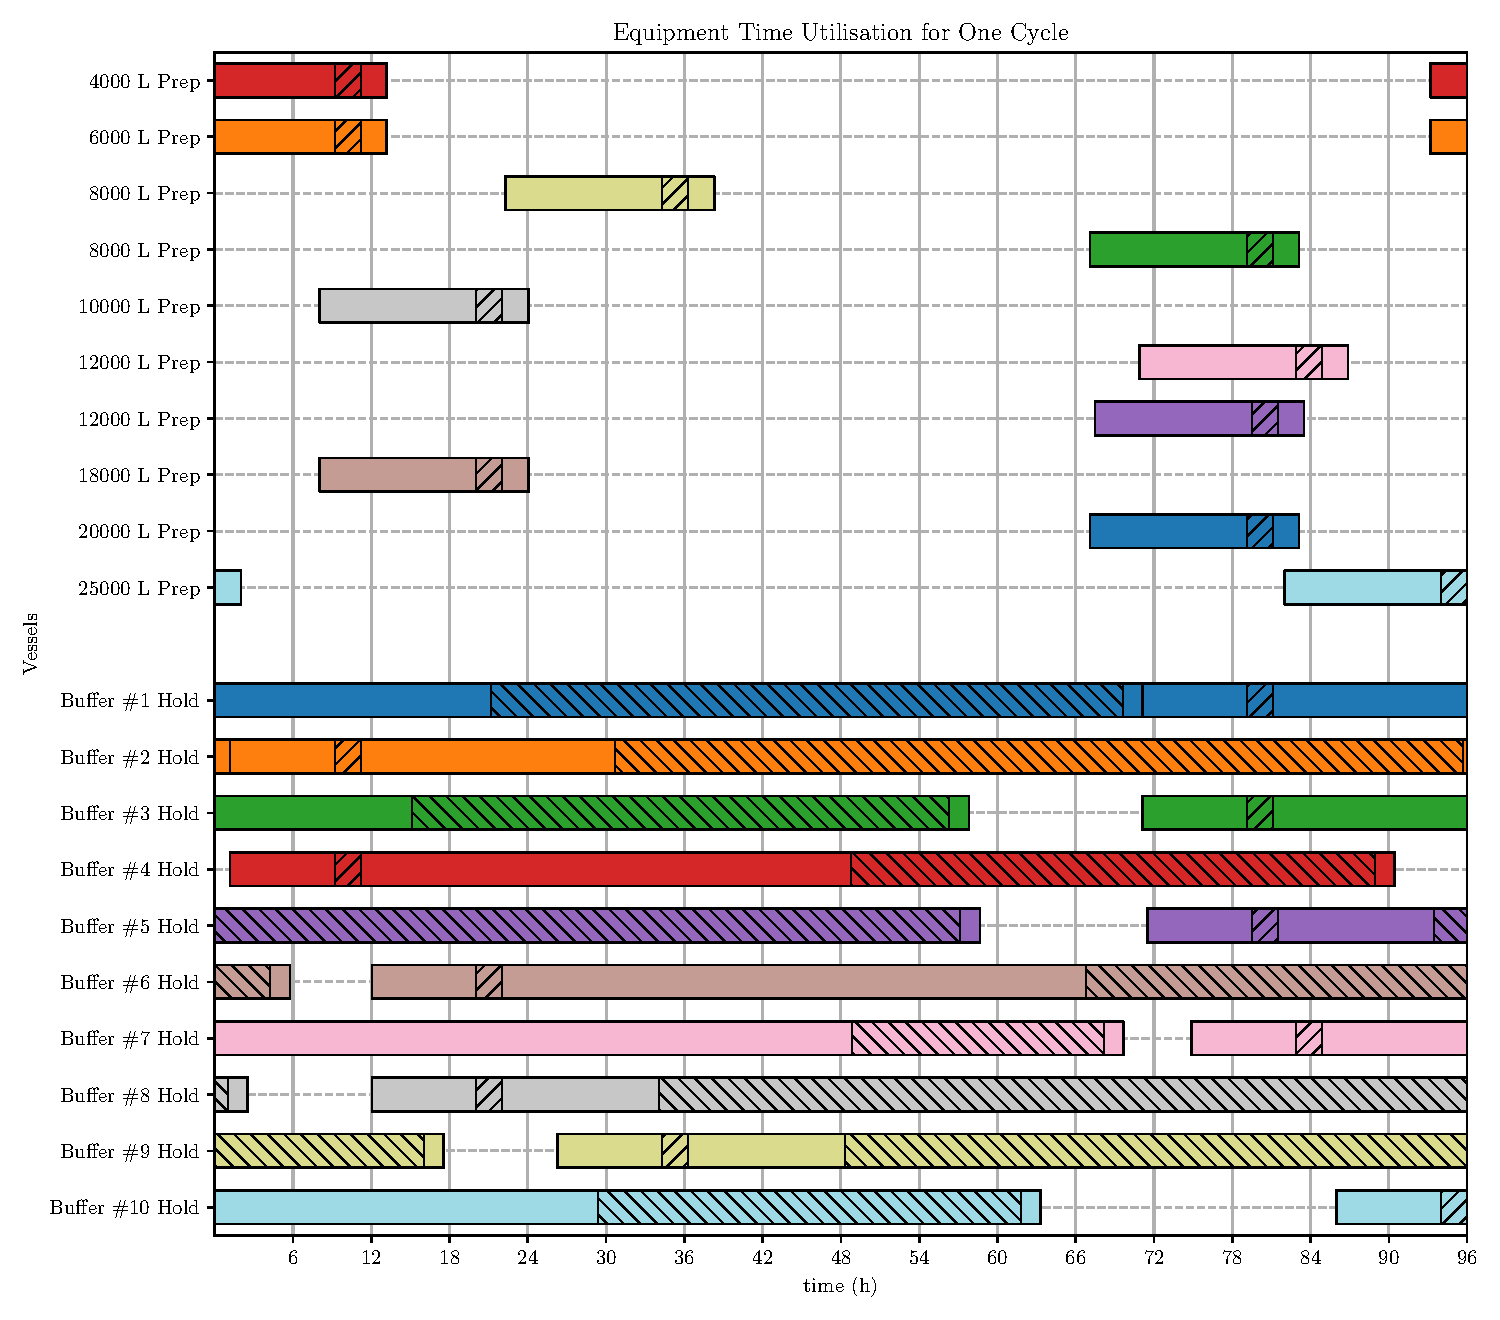
\includegraphics[width=\linewidth]{./figures/plot1.pdf}
    \caption{Equipment time utilisation for random example}
    \label{fig.etu1}
\end{figure}
Each horizontal dotted line represents a piece of equipment (preparation or
hold vessels in this case).
The presence of a bar on a dotted line indicates that the respective piece of
equipment is in use.  
The hatched bars indicate transfers, as per the legend.

Transfer from a buffer hold vessel to the production process is shown as a
contiguous bar in the hold vessel, representing the
period from the start of the first use to the end of the last use of the buffer
in a given batch, although the demand from the production process may be
discontinuous.

The bars are coloured by buffer. Since the buffer hold vessels are dedicated
to particular buffers, and are named according to the buffers they contain,
the buffer hold entries serve as a legend for the colour scheme.

Note that the time window shown in \hyperref[fig.etu1]{Figure \ref*{fig.etu1}}
displays a single cycle at steady-state; the next cycle and the previous cycle
would be identical.
The offset of the single-cycle window is somewhat arbitrary; the
visible window can be thought of as a cylinder that has been cut at right a
angles to its ends and flattened out.

It should be noted also that \hyperref[fig.etu1]{Figure \ref*{fig.etu1}}
does not highlight the batches to which the procedures belong.
The entire downstream process may take more than one cycle to complete, so the
window visible in the plot could be showing buffer preparation and hold
procedures from several successive batches.

The visual output of an equipment time utilisation plot provides a useful
method for validating results.
As the model detailed in 
\hyperref[C.methodology]{Chapter \ref*{C.methodology}} was being developed,
such plots were a useful way of highlighting logical flaws or bugs in the code.
With the finished model, such plots are a useful tool for convincing
colleagues and clients that a proposed vessel selection is indeed feasible.

\section{Solution Duration}\label{S.soltime}
\subsection{Variation of Problem Size}\label{SS.buffcount}
Using the parameters data set given in 
\hyperref[tbl.parameters]{Table \ref*{tbl.parameters}} and the vessels data set
given in \hyperref[tbl.vessel]{Table \ref*{tbl.vessel}}, the time taken for
the CPLEX solver to reach a feasible solution was evaluated for a range of 
randomly-generated buffer data sets of different sizes.

The runs were carried out on a computer with \SI{16}{\giga\byte} of RAM and an
Intel 3770K processor (four physical cores; eight virtual cores, running at
\SIrange{3.5}{3.9}{\GHz}).
The operating system was Arch Linux 64 bit (rolling release).
It was note that the CPLEX solver uses multi-threading effectively, as all
eight virtual cores were running at \SI{100}{\%} fairly consistently during the
runs (the usage tended to dip slightly at the start and end of each run).
RAM usage during the runs was below \SI{1}{\giga\byte}, so memory shortage was
not a factor in the solution durations.

\begin{figure}
    \label{fig.timing}
    \centering
    \includegraphics[width=\linewidth]{./figures/timing.pdf}
    \caption{Solution time as a function of buffer count}
\end{figure}

For a set of problem sizes (i.e.\ values of $N$), 100 random data sets
were generated for each problem size and the solution durations were recorded.
A box plot of the durations is shown in 
\hyperref[fig.timing]{Figure \ref*{fig.timing}}.
A total of \num{1000} runs were performed to generate
\hyperref[fig.timing]{Figure \ref*{fig.timing}} and for each run, an optimal
solution was found.
Note that there are several slow outliers for each problem size.
In the case of $N=20$, the highest outlier is approximately two
orders of magnitude greater than the mean duration, indicating a high degree
of variability.

Such variability in solution duration is not uncommon in MILP problems.
Methods for solving problems with binary variables necessarily involve some
searching through large binary trees, where search time can vary greatly
depending on the location of the optimum result and the search strategy.

\subsection{Comparison of Solvers}\label{SS.solvers}
A similar analysis to that carried out in
\hyperref[SS.buffcount]{Section \ref*{SS.buffcount}} was attempted with the
Cbc and GLPK solvers.
The results are shown in \hyperref[fig.timings]{Figure \ref*{fig.timings}}.
Each point represents the mean duration of 100 runs of a particular problem
size with a particular solver.

Both Cbc and GLPK were found to be considerably slower than CPLEX.

The GLPK solver is only capable of running single-threaded so cannot take
advantage of a multi-threaded processor.
It was the fastest at solving the trivial two-buffer problem, but showed the
steepest rate of solution time increase with increasing number of buffers.
At a size of $N=8$, GLPK showed massive variation in solution time, with
solutions ranging from less than 10 seconds to over 8 hours.  As a result,
only data points for $N=6$ and below are shown for GLPK.

The Cbc solver had better performance but had reliability issues; on three
random runs out of 100, with a problem size of $N=10$, Cbc was taking several
orders of magnitude longer than the mean to obtain a solution, so those runs
were halted.
While the CPLEX and GLPK solvers were called with no arguments, the
\texttt{threads=8} argument was passed to the Cbc solver to get it to use all
virtual cores on the computer (CPLEX uses all virtual cores by default and GLPK
only operates as a single thread).

CPLEX proved robust over the range $2 \le N \le 20$.

\begin{figure}
    \label{fig.timings}
    \centering
    \includegraphics[width=\linewidth]{./figures/timings.pdf}
    \caption{Solution time as a function of buffer count}
\end{figure}

Note that the data in \hyperref[fig.timings]{Figure \ref*{fig.timings}}
indicate that solution time is exponential in $N$, which is to be expected for
an \textbf{NP}-hard optimisation problem.

\subsection{Real-World Data}\label{SS.realworld}
The model was applied to (obfuscated) data from two real-world data sources.
In both cases, CPLEX found feasible solutions in under one minute.
The data and results for both real-world examples are recorded in an appendix
to this report.


%   MSc Business Analytics Dissertation
%   Format based on skeleton template provided as part of module MIS40750
%
%   Title:     Optimising the design of buffer preparation in bioprocessing
%              facilities
%   Author:    Sean Tully
%
%   Chapter 6: Discussion
%
%   Change Control:
%   When     Who   Ver  What
%   -------  ----  ---  --------------------------------------------------------
%   06Jun16  ST    0.1  Begun 
%

\chapter{Discussion}\label{C.discussion}

\section{Introduction}\label{S.intro6}

In this chapter we examine \ldots

%TODO
\textbf{TODO: interesting things about the results}

%TODO
\textbf{TODO: scope for further work}

%   MSc Business Analytics Dissertation
%
%   Title:     Aaa Bbbbbbb Cccccccccc
%   Author(s): Xxxxxx Xxxxxxxxx and Yyy Yyyyyyyyy
%
%   Chapter 7: Conclusions and Future Research
%
%   Change Control:
%   When     Who   Ver  What
%   -------  ----  ---  --------------------------------------------------------------
%   11Feb11  AB    0.1  Begun 
%

\chapter{Conclusions and Future Research}\label{C.Conclusions.Future.research}

\begin{quote}
\textit{-- That's a most foolhardy remark, he said sharply, because the nerve-strings and 
the sheep's head itself are whirling into the same bargain and you can cancel out one whirl 
against the other and there you are --- like simplifying a division sum when you have fives 
above and below the bar.}

\textit{-- To say the truth I did not think of that.} 

\textit{-- Mollycules is a very intricate theorem and can be worked out with algebra but you 
would want to take it by degrees with rulers and cosines and familiar other instruments and 
then at the wind-up not believe what you had proved at all.  If that happened you would have 
to go over it till you got a place where you could believe your own facts and figures as 
exactly delineated from Hall and Knight's Algebra and then go on again from that particular 
place till you had the whole pancake properly believed and not have bits of it half-believed 
or a doubt in your head hurting you like when you lose the stud of your shirt in the middle 
of the bed.} 

\hspace{2cm}--- Flann O'Brien, \emph{The Dalkey Archive}
\end{quote}


\section{Introduction}\label{S.Concl.intro}

The significance of \ldots



%% Back matter (loose ends: continue arabic page numbering)
\backmatter

%%   Appendices, if any: there will almost certainly be one or more.
%%   This is where you put material which the reader may like to refer to but 
%%   which might break the train of thought in the thesis proper.  Large tables,
%%   etc might go here.  You may also include program code if not too long: say
%%   a few important chunks.  But the majority of this should just be put on the
%%   accompanying CD/DVD. \include appendix/ces as it/they will be big enough to
%%   justify its/their own ``chapter(s)''
\cleardoublepage
%\appendix          %%%%% Removed this line and next two - ST   
%\addappheadtotoc         % adds a separating entry to the TOC, saying Appendices
%\noappendicestocpagenum  % ensures there is no page number after that TOC 
%                          separating entry
% It may happen that the first appendix (e.g., Detailed Tables) appears before
% the "Appendices" line in the table of contents.  If so, edit thesis.toc and
% move the Appendices line there above the first appendix, then re-run LaTeX to 
% get the thesis.dvi file right.  You may have to repeatedly do this every time 
% you LaTeX!
%\cleardoublepage    %%%%% Removed - ST
%%   MSc Business Analytics Dissertation
%   Format based on skeleton template provided as part of module MIS40750
%
%   Title:     Optimising the design of buffer preparation in bioprocessing
%              facilities
%   Author:    Sean Tully
%
%   Appendix 1: Running the Model
%
%   Change Control:
%   When     Who   Ver  What
%   -------  ----  ---  --------------------------------------------------------
%   06Jun16  ST    0.1  Begun 
%
\addappheadtotoc
\chapter{Program installation and usage}\label{C.Appendix1}
\begin{itemize}
\item
Python should be installed, along with the third-party python libraries
listed in \hyperref[tbl.libs]{Table \ref*{tbl.libs}}.
Note that the code in \texttt{model.py} requires version 3.3 (or newer) of
python.
The specific versions of all packages and libraries mentioned in
\hyperref[S.implementation]{Section \ref*{S.implementation}}
were found to be compatible.
It may be possible that breakages occur with other versions.
The pyenv package may be required to ensure the correct version of python is
available to the modelling code.
Optionally, additional
MILP solvers may be installed, such as those mentioned in
\hyperref[SS.impl1]{Section \ref*{SS.impl1}}.

\item
Clone the model repository by running the following from the terminal:
\texttt{\$ mkdir -p \textasciitilde/git\\
        \$ cd \textasciitilde/git\\
        \$ git clone \url{https://github.com/multipitch/dissertation}}

\item
To make the \texttt{runmodel} executable available to the user, it must be
appended to the user's \texttt{PATH} environment variable.
This can be achieved, for the active terminal session, by running the following
from within the terminal:

\texttt{\$ export PATH=\$PATH:<location>}

where \texttt{<location>} is the path to the directory containing
\texttt{runmodel} e.g.

\texttt{\$ export PATH=\$PATH:\textasciitilde/git/dissertation/src}

The above redefinition of \texttt{PATH} can be made permanent by appending the
command to e.g.\ the user's \texttt{\textasciitilde/.bashrc} file.

\item
To run using the default settings, given a directory containing valid input data
 (\texttt{buffers.csv},
\texttt{vessels.csv} and \texttt{parameters.ini} files), navigate to the
directory and run the following from the command line:

\texttt{\$ runmodel}

The above command uses PuLP's default solver (Cbc), without any arguments.
It solves for both the primary and secondary models and generates equipment
time utilisation plots for both, saving them to the directory as
\texttt{plot1.pdf} and \texttt{plot2.pdf}.

\item
Several optional parameters may be passed to the \texttt{runmodel} executable,
e.g.\ running

\texttt{\$ runmodel -s CPLEX -{}-no-secondary}

will run the model using the CPLEX solver and won't perform the secondary
optimisation.

A description of all input parameters is available by running \texttt{runmodel}
with the \texttt{-h} or \texttt{-{}-help} flags.

\item
Sample data is available in the examples directory of the repository.
The command below gives an example of how to carry out a run on one of the 
sample data sets:

\texttt{\$ runmodel -P ~/git/dissertation/examples/random/}
\end{itemize}
 %%%%% Removed - ST
%%   MSc Business Analytics Dissertation
%   Format based on skeleton template provided as part of module MIS40750
%
%   Title:     Optimising the design of buffer preparation in bioprocessing
%              facilities
%   Author:    Sean Tully
%
%   Appendix 2: program code
%
%   Change Control:
%   When     Who   Ver  What
%   -------  ----  ---  --------------------------------------------------------
%   06Jun16  ST    0.1  Begun 
%

\chapter{Program code}\label{C.Appendix2}

Xyz etc
 %%%%% Removed - ST
% and so on

%%   Endnotes (if needed)

%%   Glossary of terms
%%   \include this as it may be big enough to justify its own ``chapter''
%\cleardoublepage                         %%%%% Removed - ST
%\addcontentsline{toc}{chapter}{Glossary} %%%%% Removed - ST
%%   MSc Business Analytics Dissertation
%   Format based on skeleton template provided as part of module MIS40750
%
%   Title:     Optimising the design of buffer preparation in bioprocessing
%              facilities
%   Author:    Sean Tully
%
%   Glossary
%
%   Change Control:
%   When     Who   Ver  What
%   -------  ----  ---  --------------------------------------------------------
%   06Jun16  ST    0.1  Begun 
%

\chapter*{Glossary}\label{C.glossary}

Entries are listed in alphabetical order.  

                       %%%%% Removed - ST

%%   Bibliography (References)
\cleardoublepage
\addcontentsline{toc}{chapter}{Bibliography}
\bibliographystyle{mscBA} % the BibTeX style file to use %was mscBA
\bibliography{thesis}     % the BibTeX database file to use 

\cleardoublepage
\addcontentsline{toc}{chapter}{List of Notation}
%   MSc Business Analytics Dissertation
%   Format based on skeleton template provided as part of module MIS40750
%
%   Title:     Optimising the design of buffer preparation in bioprocessing
%              facilities
%   Author:    Sean Tully
%
%   List of Notation
%
%   Change Control:
%   When     Who   Ver  What
%   -------  ----  ---  --------------------------------------------------------
%   06Jun16  ST    0.1  Begun
%

\chapter*{List of Notation}\label{C.notation}

\vspace{0.5cm}

{\renewcommand{\arraystretch}{0.9}

\begin{longtabu} to \textwidth {X[-1,l] X[1,l]<{\strut} X[-1,r]}
    \tb{Symbol} & \tb{Description} & \tb{Ref}\\\hline
    \endhead
    $\boldsymbol{a}_{nk}$ & boolean; buffers $n$ and $k$ prepared in same
    vessel & \ref{SS.constr6}\\
    $c_{m}$ & (relative) cost of vessel $m$ & \ref{S.vesseldata}\\
    $f_{\mathit{MAXUSE}}$ & buffer maximum use time ratio 
        & \ref{SS.randomdata}\\
    $f_{\mathit{MINFILL}}$ & vessel minimum fill ratio & \ref{S.parameters}\\
    $f_{\mathit{MINUSE}}$ & buffer minimum use time ratio 
        & \ref{SS.randomdata}\\
    $f_{\mathit{UTIL}}$ & preparation slot maximum utilisation ratio
        & \ref{S.parameters}\\
    $k$ & secondary buffer index $\left( k \in N, k \ne n \right)$
        & \ref{SS.schedintro}\\
    $m$ & vessel size index $\left( m \in M \right)$ & \ref{S.vesseldata}\\
    $n$ & buffer index $\left( n \in N \right)$ & \ref{S.bufferdata}\\
    $p$ & slot index $\left( p \in P \right)$ & \ref{S.slots}\\
    $\boldsymbol{q}_{n}$ & boolean; 
        $t_{\mathit{USE},n} - \boldsymbol{z}_{n} < 0$ & \ref{SS.prepreftimes}\\
    $\boldsymbol{r}_{n}$ & boolean; 
        $t_{\mathit{USE},n} - \boldsymbol{z}_{n} < 0$ & \ref{SS.cyclic}\\
    $\boldsymbol{s}_{n}$ & boolean; 
        $t_{\mathit{USE},n} - \boldsymbol{z}_{n} < 0$ & \ref{SS.cyclic}\\
    $t_{\mathit{LOWER},n}$ & lower bound of feasible scheduling region for all
        buffers $k > n$ with respect to buffer $n$ & \ref{SS.cyclic}\\
    $t_{\mathit{UPPER},n}$ & upper bound of feasible scheduling region for all
        buffers $k > n$ with respect to buffer $n$ & \ref{SS.cyclic}\\
    $t_{\mathit{PREP},k}$ & preparation reference time for buffer $k$ 
        & \ref{SS.prepreftimes}\\
    $t_{\mathit{PREP},n}$ & preparation reference time for buffer $n$ 
        & \ref{SS.prepreftimes}\\
    $t_{\mathit{USE},n}$ & buffer $n$ time of first use, normalised
        & \ref{S.bufferdata}\\
    $t_{\mathit{USE},n}^{*}$ & buffer $n$ time of first use, unnormalised 
        & \ref{S.bufferdata}\\
    $\Delta t_{\mathit{FEAS}}$ & maximum feasible buffer use duration
        & \ref{SS.randomdata}\\
    $\Delta t_{\mathit{HOLD,MAX}}$ & maximum allowable buffer hold duration
        & \ref{S.parameters}\\
    $\Delta t_{\mathit{HOLD,MIN}}$ & minimum allowable buffer hold duration
        & \ref{S.parameters}\\
    $\Delta t_{\mathit{HOLD,POST}}$ & duration of post-use operations in buffer
        hold procedures & \ref{S.parameters}\\
    $\Delta t_{\mathit{HOLD,PRE}}$ & duration of operations prior to receiving
        buffer in buffer hold procedures & \ref{S.parameters}\\
    $\Delta t_{\mathit{PREP,PRE}}$ & duration of operations prior to
        transferring out buffer in buffer preparation procedures & 
        \ref{S.parameters}\\
    $\Delta t_{\mathit{PREP,POST}}$ & duration of operations post transferring
        out buffer in buffer preparation procedures & \ref{S.parameters}\\
    $\Delta t_{\mathit{PREP}}$ & total duration of buffer preparation
        procedure & \ref{SS.constr4}\\
    $\Delta t_{\mathit{USE},n}$ & duration of use of buffer $n$ 
        & \ref{S.bufferdata}\\
    $\Delta t_{\mathit{TRANSFER}}$ & duration of transfer from buffer
        preparation vessel to buffer hold vessel & \ref{S.parameters}\\
    $\boldsymbol{u}_{n}$ & boolean; single feasible scheduling window for 
        buffer $k > n$ with respect to buffer $n$ & \ref{SS.cyclic}\\
    $\boldsymbol{v}_{nk}$ & boolean; feasible scheduling window for buffer
        $k > n$ is before buffer $n$ preparation procedure & \ref{SS.cyclic}\\
    $\boldsymbol{w}_{nkp}$ & boolean; distinct buffers $n$ and $k$ are both
        made in slot $p$ & \ref{SS.constr6}\\
    $\boldsymbol{x}_{np}$ & boolean; buffer $n$ is prepared in slot $p$
        & \ref{SS.constr1}\\
    $\boldsymbol{y}_{mp}$ & boolean; a vessel of size $m$ is in slot $p$
        & \ref{S.objfn}\\
    $\boldsymbol{z}_{n}$ & buffer $n$ hold duration & \ref{SS.constr5}\\
    $M$ & Set of vessel sizes & \ref{S.vesseldata}\\
    $\mathcal{M}$ & number of vessel sizes & \ref{S.vesseldata}\\
    $N$ & Set of buffers & \ref{S.bufferdata}\\
    $\mathcal{N}$ & number of buffers & \ref{S.bufferdata}\\
    $P$ & Set of slots & \ref{S.slots}\\
    $\mathcal{P}$ & number of slots & \ref{S.slots}\\
    $T$ & process cycle time (start--to--start duration) & \ref{S.parameters}\\
    $U_{n}$ & volume of buffer $n$ to be preapred & \ref{S.bufferdata}\\
    $V_{m}$ & maximum working volume of vessel size $m$ & \ref{S.vesseldata}\\
    $V_{\mathit{MAX}}$ & largest maximum working volume of available vessel
        sizes & \ref{SS.constr3}\\
    $\boldsymbol{Y}$ & secondary objective; sum of buffer hold times,
        given minimal total vessel cost & \ref{SS.goal}\\
    $\boldsymbol{Z}$ & primary objective; total vessel cost & \ref{S.objfn}\\
    $Z^{\prime}$ & minimal total vessel cost & \ref{SS.goal}\\
\end{longtabu}

}

Notes:

Decision variables and objective function values are in 
$\boldsymbol{\mathit{bold}}$ text.

Subscripts in lower-case represent indices.
Subscripts in upper-case are descriptive.
Both subscript types may be used simultaneously, e.g. in the case of
$t_{USE,n}$.

A prime suprescript denotes an optimum value, e.g. $Z^{\prime}$.

Greek letters are used throughout the text as `throwaway' variables, to
explain certain concepts and are not included in the list of notation.


%%   Index
%\cleardoublepage                      %%%%% Removed - ST
%\addcontentsline{toc}{chapter}{Index} %%%%% Removed - ST
%\printindex                           %%%%% Removed - ST

\end{document}
